\title{Optimisations for finite state Mealy automata}
\author{
        Aleksander Mendoza \\
                Department of Mathematics and Computer Science\\
        Adam Mickiewicz University\\
        Poznan, \underline{Poland}         
}
\date{\today}

\documentclass[12pt]{article}
\usepackage{tikz}
\usepackage[utf8]{inputenc}
\usepackage[T1]{fontenc}
\usepackage{lmodern}
\usepackage{amsfonts}
\usepackage{mathrsfs}
\usepackage{centernot}
\usepackage{listings}
\usepackage{mathtools}
\usepackage{xcolor}
\usepackage{amsmath}
\usepackage{amssymb}

\begin{document}
\maketitle
\lstset{
	basicstyle=\ttfamily,
	mathescape
}

\part{Foundations}
\section{Definitions}
Standard definition of Mealy machine is provided as $(Q,q_0,\Sigma,\Gamma,\delta,G,F)$ where $Q$ is set of states, $q_0 \in Q$ is the initial state, $\Sigma$ and $\Gamma$ are respectively input and output alphabets, $\delta: Q \times \Sigma \rightarrow Q$ is the transition function , $G: Q \times \Sigma \rightarrow \Gamma$ it specifies output associated with each transition and $F$ is the set of accepting states. Finite state automaton is defined similarly as $(Q,q_0,\Sigma,\delta, F)$ but it doesn't have any output. It's possible to extend both machines to non-deterministic models by adding $\epsilon$ to transition and/or output functions as in 
$\delta: Q \times (\Sigma \cup \{\epsilon\})\rightarrow Q$ and $G: Q \times (\Sigma \cup \{\epsilon\})\rightarrow (\Gamma \cup \{\epsilon\})$.  We can show that introducing non-determinism this way is equivalent to defining it as $\delta: Q \times (\Sigma \cup \{\epsilon\})\rightarrow P(Q)$ for finite state automata (and $\delta: Q \times (\Sigma \cup \{\epsilon\}) \rightarrow P(Q \times \Gamma)$ for Mealy machines) but in our case, just adding epsilon is enough and will make things simpler later. You can treat finite state machines as predicates on formal languages. For instance if $P$ is an automaton, then $\forall_{x\in \Sigma^*} P(x) \iff P \textrm{ accepts }x$. Mealy machines on the other hand, can be interpreted as relations on languages. Let's say $M$ is a Mealy machine, then $\forall_{x\in\Sigma^*, y \in \Gamma^*} M(x,y) \iff M \textrm{ produces } y \textrm{ as one of it's outputs, on input } x$. So in a sense, $P$ is equivalent to some subset of $\Sigma^*$, while $M$ is equivalent to some subset of $\Sigma^* \times \Gamma^*$. If additionally $M$ is a (partial) function ( it holds that $\forall_{x\in\Sigma^* , y,z \in \Gamma^* } M(x,y) \wedge M(x,z) \implies y=z$ ), then we can write $M(x)=y$ instead of $M(x,y)$. It's important to remember that there  might exist many different automata inducing the same language or relation on languages. Therefore we shall write $P_0 = P_1$ to mean $\forall_{x\in\Sigma^*} P_0(x) \iff P_1(x)$ even when $P_0$ and $P_1$ have different structures. Similarly $M_0 = M_1$ when $\forall_{x \in \Sigma^* , y\in\Gamma^*}M_0(x,y) \iff M_1(x,y)$.  We define two projections for Mealy machines: 
\begin{itemize}
	\item input projection $\pi_0(M) = P$ such that $\forall_{x\in\Sigma^*} (\exists_{y\in\Gamma^*}M(x,y) ) \iff P(x) $
	\item output projection  $\pi_1(M) = P$ such that $\forall_{y\in\Gamma^*} (\exists_{x\in\Sigma^*}M(x,y) ) \iff P(y) $
\end{itemize} 
We also define $\hat{\delta} : Q \times \Sigma^* \rightarrow Q$ to be extended transition function: \\
$\hat{\delta}(q,\epsilon) = q$ \\
$\hat{\delta}(q,s's) = \hat{\delta}(\delta(q,s'),s)$ where $s' \in \Sigma$\\
And similarly $\hat{G}:Q\times\Sigma^*\rightarrow\Gamma^*$ is the extended output function: \\
$\hat{G}(q,\epsilon) = \epsilon$ \\
$\hat{G}(q,s's) = G(q,s')\hat{G}(\delta(q,s'),s)$ where $s' \in \Sigma$\\
Deterministic and non-deterministic automata are equivalent in their power to recognise formal languages, however non-deterministic Mealy machines have more expressive power to relate two formal languages with each other. Let's consider several cases with help of pumping lemma. 

\paragraph{Pumping lemma for regular languages}
If $L$ is a regular language then there exists $p\ge1$  such that for all $l \in L$ where $\vert l \vert \ge p$ , can be decomposed to $l = xyz$ that satisfy the following conditions:
\begin{itemize}
	\item $\vert y \vert \ge 1$ 
	\item $\vert xy \vert \le p$ 
	\item $\forall_{n\in \mathbb{N}}  xy^nz \in L$ 
\end{itemize}

\paragraph{Deterministic single-output Mealy machines} Determinism guarantees us that for given machine $M$, the relation $M \subset \Sigma^* \times \Gamma^*$ is in fact a function $M \subset \Sigma^* \rightarrow \Gamma^*$. For any input $x \in \Sigma^*$, there exists only one output $y\in \Gamma^*$ such that $M(x,y)$. Moreover because $G: Q \times \Sigma \rightarrow \Gamma$ always returns exactly one element from $\Gamma$, we can be sure that $\vert x\vert = \vert y\vert$. We can apply pumping lemma to both input and output projection of $M$. We can also go further and fuse both $\Sigma$ and $\Gamma$ using Cantor's pairing function into a new alphabet $\Sigma \times \Gamma$ and then apply pumping lemma to it. Another important feature is that prefixes must match: \\
$\forall_{x,y\in \Sigma^*} \exists_{a \in \Gamma^* } M(xy)=M(x)a$ \\
This is a very problematic restriction. It implies that relation \\
$M(x) = \begin{cases}
0^{\vert x \vert} & \mbox{if } \vert x \vert \mbox{ is multiple of 2}   \\
1^{\vert x \vert}& \mbox{otherwise} 
\end{cases}$ \\
is not possible, because $M(a) = 1$, $M(aa) = 00$  for $a \in \Sigma$ and $0,1 \in \Gamma$. However, it is worth noticing that relations: \\
$M_0(x) = \begin{cases}
0^{\vert x \vert} & \mbox{if } \vert x \vert \mbox{ is multiple of 2}   \\
\mbox{ reject otherwise} 
\end{cases}$ \\
and  \\
$M_1(x) = \begin{cases}
1^{\vert x \vert} & \mbox{if } \vert x \vert \mbox{ is not multiple of 2}   \\
\mbox{ reject otherwise} 
\end{cases}$ \\
are valid. The class of relations defined by this model is not closed under union.

\paragraph{Deterministic multi-output Mealy machines} This model is defined as above except that $G: Q \times \Sigma \rightarrow \Gamma^*$. This breaks the guarantee that $\vert x\vert = \vert y\vert$. Now $y$ can be of any length. However, you can still apply pumping lemma to both projections of $M$. You just cannot apply it to fused alphabet $\Sigma \times \Gamma$. Moreover, the prefix restriction still holds: \\
$\forall_{x,y\in \Sigma^*} \exists_{a \in \Gamma^* } M(xy)=M(x)a$ \\


\paragraph{Disjunctive Mealy machines} They are defined in a very different way. They can write to multiple   tapes. Output function becomes $G: Q \times \Sigma \times T \rightarrow \Gamma^*$ where $T$ is a finite set of tapes. $F$ is no longer a set but a function $F: Q \rightarrow T \cup \{\emptyset\}$ (or alternatively you could treat it as partial function $F: Q \rightarrow T$). This model works by reading consecutive input characters $s \in \Sigma$ , and transitioning from state $q\in Q$ to $\delta(q,s)$. On each transition automaton writes  $G(q,s,t)$ to every tape $t \in T$. When input reaches end and automaton halts in state $q$, the returned output should be taken from $F(q)$. In cases when $F(q) = \emptyset$ , the automaton rejects. This model is still deterministic but multiple tapes allow it to break the rule of matching prefixes.
Also, the projections $\pi_0$ and $\pi_1$ still apply but additionally we define projection $\pi_t$ for every tape $t$. More formally:\\
$\pi_t(M) = P$ such that $\forall_{y\in\Gamma^*} (\exists_{x\in\Sigma^*} M(x,y) \wedge F(\hat{\delta}_M(q_{0M},x))=t) \iff P(y)$

\paragraph{Functional Mealy machines} This is an even further extension of disjunctive Mealy machines. Now the tapes are no longer fixed. Instead every state has their own set of them. And every transition translates tapes of one states onto tapes of some other. Therefore it's better to think of is as memory cells associated with each states rather than actual tapes of whole automaton. Transitions copy contents of one cell into another, while also append some additional output. Here is a formal definition: \\
$T$ is the set of cells. \\
$\delta : Q \times \Sigma \rightarrow Q$ is the plain transition function between states. \\
$\gamma : Q \times \Sigma^* \times T \rightarrow (\Gamma^*\cup\{\emptyset \})$ is called context function. At any given time each cell from every state is either empty  or contains some string from $\Gamma^*$. We can retrieve those strings using $\gamma$. For instance $\gamma(q_4,010010,t_3)$ stands for contents of cell $t_3$ of state $q_4$ after reading input $010010$. \\
$G : Q \times \Sigma \times T \rightarrow  \Gamma^*\times T$ is the \underline{partial} transition function between memory cells.  $G(q,s,t') = (s',t)$ tells you to copy contents of  cell $t$ at state $q$, append $s'$ and put resulting string  in cell $t'$ of state $\delta(q,s)$.  \\
$F : Q \rightarrow (T \cup \{\emptyset\})$ is the accepting function that tells us which memory cell to take the output from. \\
$(q_0,\gamma(q_0,\epsilon)) : Q \times (T \rightarrow \Gamma^*)$ is the initial state along with some initial assignment to each memory cell. Therefore $\gamma(q_0,\epsilon,t)$ for any $t\in T$ is initially set.\\
The evaluation of such automaton follows this simple rule: \\
Let $G(q,s,t') = (s',t')$ then for all $z\in\Sigma^*$ \\
$\gamma(\delta(q,s),zs,t')= \gamma(q,z,t) s' $ \\
whereas if $\forall_{t'\in T} G(q,s,t') = \emptyset$ then  $\gamma(\delta(q,s),zs,t') = \emptyset$.
Also notice that if $\gamma(q,z,t) = \emptyset$ then $\gamma(q,z,t) s' = \emptyset$, because concatenation with empty language yields empty language too. \\
Let's illustrate the process with an example: \\
$\Sigma = \{a\}, \Gamma=\{0,1\}, T=\{A,B,C,D,E\}$
\begin{center}
	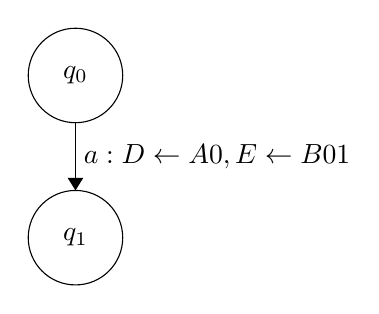
\begin{tikzpicture}[scale=0.2]
	\tikzstyle{every node}+=[inner sep=0pt]
	\draw [black] (13.9,-11.2) circle (3);
	\draw (13.9,-11.2) node {$q_0$};
	\draw [black] (13.9,-21.5) circle (3);
	\draw (13.9,-21.5) node {$q_1$};
	\draw [black] (13.9,-14.2) -- (13.9,-18.5);
	\fill [black] (13.9,-18.5) -- (14.4,-17.7) -- (13.4,-17.7);
	\draw (14.4,-16.35) node [right] {$a:D\leftarrow A0,E\leftarrow B01$};
	\end{tikzpicture}
\end{center}
The notation $a:D\leftarrow A0,E\leftarrow B01$ stands for $\delta(q_0,a) = q_1$ and \\
$G(q_0,a,D) =(0,A)$ \\
$G(q_0,a,E) = (01,B)$ \\
(the rest is undefined because G can be partial)\\
 Let's say you are in state $q_0$ with memory cells containing $\gamma(q_0,z,A)=001$, $\gamma(q_0,z,B)=\epsilon$, $\gamma(q_0,z,C)=11$. Then after transitioning over letter $a$, you will reach state $q_1$ with memory cells $\gamma(q_1,za,D)=\gamma(q_0,z,A)0=0010$ and $\gamma(q_1,za,E)=\gamma(q_0,z,B)01=01$. Notice that contents of $\gamma(q_0,z,C)$, $\gamma(q_0,z,D)$ and $\gamma(q_0,z,E)$ are not copied anywhere so they get lost.  Contents of $\gamma(q_1,za,A)$, $\gamma(q_1,za,B)$, $\gamma(q_1,za,C)$ are equal $\emptyset$.

\paragraph{Non-deterministic Mealy machines} This model allows for greatest flexibility. $M \subset \Sigma^* \times \Gamma^*$ does not have any restrictions apart from the requirement that both input and output language must be regular. Furthermore, we can use epsilons to associate one input with multiple outputs. In fact, there could be infinitely many of them if epsilons create a loop at some point. 


\paragraph{Moore machines}
This model is largely equivalent to Mealy machines. The only difference is that output function has form of $G:Q\rightarrow\Gamma$ so it depends solely on state. You can convert every variant of Mealy machine to corresponding Moore machine. Here is a quick comparison:
\begin{center}
	\begin{table}[!htbp]
		\begin{tabular}{|l|l|l|}
			\hline
			variant          & Mealy & \multicolumn{1}{c|}{Moore} \\ \hline
			single-output    & $G:Q\times\Sigma\rightarrow\Gamma$     & $G:Q\rightarrow\Gamma$                           \\ \hline
			multi-output     & $G:Q\times\Sigma\rightarrow\Gamma^*$      & $G:Q\rightarrow\Gamma^*$                           \\ \hline
			disjunctive       & $G:Q\times\Sigma\times T\rightarrow\Gamma$      & $G:Q\times T\rightarrow\Gamma$                             \\ \hline
			nondeterministic &  $G:Q\times(\Sigma\cup\{\epsilon\})\rightarrow(\Gamma\cup\{\epsilon\})$     & $G:Q\rightarrow(\Gamma\cup\{\epsilon\})$                     \\ \hline
		\end{tabular}
	\end{table}
\end{center}
Conversion from  Mealy to Moore comes at the expense of adding a lot of new states (therefore Mealy machines are generally more compact). 
Let $M$ be a Mealy machine, and $N$ be Moore machine. General pattern for conversion algorithm looks like this:

For every $q\in Q_M$ and $s\in\Sigma$, put $q_s\in Q_N$ and simulate $\delta_M(q,s)=q'$ as $\forall_{t\in\Sigma}\delta_N(q_t,s)=q'_s$ along with $G_M(q,s)=s'$ as $G_N(q_s) = s'$. Depending on variant of machine, this might need some slight modifications.

You can also perform conversion the other way around but unfortunately not for every variant. In case of deterministic Mealy machines, it's impossible to express mappings for $\epsilon$, while deterministic Moore machines can do it easily (the initial state can be marked as accepting state and we can associate arbitrary output with it even without reading any input).

Another advantage of Moore machines is that we can look at their output in two ways. We can accumulate output printed by every state and therefore the disjunctiveity resembles Mealy machines very much. However, the second approach is to ignore what is printed at all intermediate outputs and only focus on the output of final state. Therefore we can define two variants of extended output functions. \\
First is Mealy-style output: \\
$\hat{G}(q,\epsilon) = G(q)$ \\
$\hat{G}(q,s's) = G(q)\cdot\hat{G}(\delta(q,s'),s)$ where $s' \in \Sigma$, $s\in\Sigma^*$ and $\cdot$ is string concatenation \\
Second is $\hat{\delta}$-style output: \\
$\check{G}(q,s) = G(\hat{\delta}(q,s))$\\


Unfortunately Moore machines are not the topic of this paper so we won't delve  into details. We only need them to present certain property of disjunctive Mealy machines. 


\section{Classes of language relations} As mentioned above, Mealy machines represent some class of relations on languages. A relation $R \subset \Sigma^* \times \Gamma^*$ is decidable if there exists some Turing machine that works on alphabet $\Sigma \cup \Gamma$ and accepts all strings in $R$ while also rejects all strings from $\overline{R}$ (we can use arbitrary way to encode pairs of strings). Of course not all relations are decidable. The most trivial example of undecidable relation is $(x,y)  \in \Sigma^* \times \{0,1\}$ where  $x$ encodes some Turing machine, and $y$ is in relation with $x$ iff $x$ halts on $y$. While Turing machines are capable of "recognizing" pairs of strings, Mealy automata can be used to "generate" the right-side element of pair for any given left-side element of pair. However, in principle both "generation" and "recognition" are just different ways to see the same phenomenon. Anything that can be generated with mealy machines can be recognized by some Turing machine. 

Let's say that we are given non-deterministic Mealy machine $M$ and input $(x,y) \in \Sigma^* \times \Gamma^*$ . The problem whether $(x,y) \in M$ is decidable, because we can simulate all non-deterministic branches of computation and reject them as soon as the length of total accumulated output equals or exceeds length of $y$. There are only finitely many strings in $\Gamma^*$ shorter or equal $y$, so we can visit all of them in finite time. Also, at any step the computation of Mealy automaton can split into only finite number of new non-deterministic branches. 

This proves that simulation of non-deterministic Mealy machines is computable. For all deterministic models the proof is even simpler. Unfortunately is doesn't work the other way around. It's not possible in general case to build Mealy machine equivalent to given Turing machine. The proof is very simple - languages accepted and generated by Mealy machines are regular. 

Apart from input and output languages being regular themselves, there are also limitations to how the relation on those languages can be structured. There exists a relation $ R \subset \Sigma^* \times \Gamma^*$
such that both $\pi_0(R)$ and $\pi_1(R)$ are regular, but despite this there is no non-deterministic Mealy automaton capable of deciding it. Proof is simple. Let $s,t\in \Gamma^*$ such that $s\ne t$ and let $R:\Sigma^* \rightarrow \Gamma^*$ such that: \\
$R(x) = \begin{cases}
t & \mbox{if }  x  \mbox{ is a valid description of Turing machine that halts on } x   \\
s & \mbox{otherwise} 
\end{cases}$ \\
Notice that $\pi_0(R) = \Sigma^*$ and $\pi_1(R) = \{s,t\}$ and both are regular. Moreover this relation is not only undecidable by Mealy machines but also not decidable by any computation model at all.

\subparagraph{Pair encodings} We can actually tell even more about the class of all relations generated by Mealy machines, but for this we need a more precise encoding for pairs of strings:
\begin{itemize}
	\item Separated pairs - Given two strings $s \in \Sigma^*$ and $t \in \Gamma^*$ we encode a pair $(s,t) \in \Sigma^* \times \Gamma^*$ as $w \in (\Sigma \cup \Gamma \cup \{\#\})^*$ where $w=s\#t^{-1}$,  $\# \notin \Sigma \cup \Gamma$ and $t^{-1}$ means "reverse of $t$". For given $R \subset \Sigma^* \times \Gamma^*$ we denote encoding of $R$ as $\mathbb{S}_\#(R) = \{w\in (\Sigma \cup \Gamma \cup \{\#\})^*: w=s\#t^{-1} \wedge (s,t) \in R \}$. Notice that for any $R$, the encoding $\mathbb{S}_\#(R)$ is unique. We say that relation $R$ is regular if there exists finite state automaton $P$ such that  $\forall_{s,t} R(s,t) \iff P(s\#t^{-1})$. Similarly $R$ is context-free if $P$ is a push-down automaton. Also, it's worth pointing out that the class of all relations is a proper subset of class of all formal languages. That's because of the restriction that every string must contain exactly one $\#$ (Given formal language $R$ over alphabet $\Theta$ you might not always be able to find isomorphism between $\Theta$ and $\Sigma \cup \Gamma \cup \{\#\}$ such that $\#$ appears in every string in $R$ exactly once).
	
	\item Interleaved pairs - Given two strings $s \in \Sigma^*$ and $t \in \Gamma^*$ we encode a pair $(s,t) \in \Sigma^* \times \Gamma^*$ as $w \in (\Sigma \cup \Gamma)^* $ where $\Sigma$ and $\Gamma$ \underline{are disjoint} , $w$ equals $s$ when you remove from $w$ all characters belonging to $\Gamma$ and similarly $w$ equals $t$ when you remove from $w$ all characters belonging to $\Sigma$. If $R \subset  \Sigma^* \times \Gamma^*$ then we denote $\mathbb{I}(R) \subset (\Sigma \cup \Gamma)^*$ as interleaved encoding of $R$. An example:\\
	Let $\Sigma = \{0,1,2\}$, $\Gamma = \{3,4,5\}$. Then pair $(001,354) \in R$ could be encoded as $030154 \in \mathbb{I}(R)$ or as $001354 \in \mathbb{I}(R)$, or $354001 \in \mathbb{I}(R)$ and so on. \\
	You can see that every pair does not have a single encoding but rather an entire class of strings becomes a valid encoding. We will say that for given encoding $\mathbb{I}(R) \subset (\Sigma \cup \Gamma)^*$ a pair $(x,y)$ belongs to $R \subset \Sigma^* \times \Gamma^*$ iff there exists at least string $\mathbb{I}(R)$ that encodes $(x,y)$. Formally $(x,y) \in R \iff \exists_{w\in\mathbb{I}(R)} w - \Sigma = y \wedge w - \Gamma = x$ where $w-X$ denotes operation of removing from string $w$ all characters from set $X$. Notice that for given $R$ there might exist multiple equivalent sets $\mathbb{I}(R)$ that encode it. Analogically to separated encoding, $R$ is regular if there exists regular $\mathbb{I}(R)$, and it is context-free if there exists context-free $\mathbb{I}(R)$. Also, it's worth pointing out that class of interleaved relations is exactly equal to class of all formal languages, because for any given formal language over alphabet $\Sigma$ you can always split $\Sigma$ into two disjoint subsets $\Sigma_0$ and $\Sigma_1$, and then interpret every string in $\Sigma^*$ as some pair in $\Sigma_0^* \times \Sigma_1^*$.
\end{itemize}
 
From now on, we will use $\mathbb{M}_1$ to refer to class of relations decidable by single-output, $\mathbb{M}_\infty$ for multi-output , $\mathbb{M}_\vee$ for disjunctive, $\mathbb{M}_\rightarrow$ for functional and $\mathbb{M}$ for non-deterministic Mealy machines. $\mathbb{REG}$ will be used to describe class of regular languages  and $\mathbb{CFG}$ for context-free languages. For given class of relations X, we will write $\mathbb{I}(X)$ to denote class of formal languages that encode relations from $X$. Formally $L  \in X \iff \mathbb{I}(L)  \in \mathbb{I}(X)$ where $L \subset \Sigma^* \times \Gamma^*$ and $\mathbb{I}(L) \subset (\Sigma \cup \Gamma)^*$. 
 
For encoding  $\mathbb{S}_\#$ it works analogically, except there is one important detail. We need to make it precise what "class of languages" stands for. A formal language is just a set of strings over some alphabet. A class of formal languages therefore is a set of sets of strings over some alphabet. There is no restriction that forces all the languages in one class to share common alphabet. In many books and papers this detail is overlooked or left implicit. Here, however, the separator character $\#$ requires us to be explicit about the alphabets and for this reason we need clear distinction between homogeneous and heterogeneous classes. 

 \subparagraph{Homogeneous and heterogeneous classes}  Formal language over finite alphabet $\Sigma$ is a subset of $\Sigma^*$. Homogeneous class of formal languages $X$ is defined as set of formal languages such that all members $L \in X$ share the same alphabet. Formally $X \subset\mathcal{P}(\Sigma^*)$ On the other hand, in a heterogeneous class of formal languages every member language could potentially use different alphabet. There are two rules of formation for such classes:
 \begin{enumerate}
	\item every homogeneous class is also a heterogeneous class
	\item if $Y$ is set (of any cardinality) of  heterogeneous classes then union	\[
	\mathop{\bigcup_{X\in Y}} X
	\] is a heterogeneous class
 \end{enumerate} 
An important thing worth noticing is that many heterogeneous classes can be seen as homogeneous classes. Suppose there are two homogeneous formal languages $X_\Sigma \subset \Sigma^*$ and  $X_\Gamma \subset \Gamma^*$. However obviously if $\Sigma$ and $\Gamma$ are finite sets then $\Sigma \cup \Gamma$ is a finite set too. Therefore the union $X_\Sigma \cup X_\Gamma$ could be a heterogeneous class derived from second rule of formation or it could be a  homogeneous class $X_\Sigma \cup X_\Gamma \subset (\Sigma \cup \Gamma)^*$. Unfortunately not all heterogeneous classes can be treated this way. The problem lies in the requirement that alphabet is finite, while the second rule of formation would allow us to have in total infinitely many disjoint alphabets (so the union of alphabets would be infinite as a result).  We can go even further and define universum $\mathcal{U}$ as the set of all finite sets, and treat it as set of all possible alphabets. Then we can define formal language universum $\top$ which is the heterogeneous class of all formal languages given by \[
\top = \bigcup_{\Sigma \in \mathcal{U}} \mathcal{P}(\Sigma^*) 
\]
Notice that $\mathbb{REG}$ and $\mathbb{CFG}$ are both heterogeneous classes in universum $\mathbb{CFG}, \mathbb{REG} \subset \top$. 

We can also extend notion of homogeneous and heterogeneous classes to relations on languages. Homogeneous class of relations $X$ over alphabets $\Sigma$ and $\Gamma$ is a subset $X \subset \mathcal{P}(\Sigma^* \times \Gamma^*)$. Heterogeneous classes of relations are constructed using analogical rules of formation as classes of languages.

After settling precise definition of classes of formal languages we can go back to the problem of separated relations. Given a class of relations $X$ (homogeneous or not), the separator character $\#$ need \underline{not} be unique or universal for all languages that are members of \underline{heterogeneous} $\mathbb{ S}(X)$. If we require all the classes to be homogeneous we can explicitly specify it as $\mathbb{ S}_\#(X)$ where $\#$ is separator character used universally by all the classes (we require that $X$ is homogeneous itself). Formally:
\begin{itemize}
	\item $\mathbb{ S}_\#(X) $ is defined as $ R \in X \iff \mathbb{ S}_\#(R) \in \mathbb{ S}_\#(X)  $ where $X$ is a homogeneous  class of relations on formal languages
	\item Given $R \subset \Sigma^* \times \Gamma^*$, $\mathbb{ S}(R)$  is defined as $\forall_{\# \notin \Sigma \cup \Gamma} \mathbb{ S}_\#(R) \in \mathbb{ S}(R)$ 
	\item $\mathbb{ S}(X)$ is defined as  $R \in X \iff \mathbb{ S}(R) \in \mathbb{ S}(X)  $
\end{itemize} 
 Notice that for any two characters $a,b \notin \Sigma \cup \Gamma$ the languages $\mathbb{S}_a(R)$ and $\mathbb{S}_b(R)$ are isomorphic (the only difference is substitution of separator $a$ for separator $b$ or vice versa). 
 
 
 
 \paragraph{$\mathbb{M}_\vee$ as Mealy-Moore union}
 Every machine in $M\in\mathbb{M}_\vee$ can be treated as union  of its projections $\pi_t(M) \in \mathbb{M}_\infty$. But writing it as \\
 $M = \bigcup_{t\in T_M} \pi_t(M)$ \\
 is abuse of notation, because the union operation is not always defined (as we will show below) for $\mathbb{M}_\infty$. What we actually mean by this notation is something like this: \\
 $M = \bigcup_{t\in T_M} \phi(\pi_t(M))$ \\
 where $\phi$ represents conversion $\mathbb{M}_\infty \rightarrow \mathbb{M}$. Let us remind the definition of tape projection: \\
 $\pi_t(M) = P$ such that $\forall_{y\in\Gamma^*} (\exists_{x\in\Sigma^*} M(x,y) \wedge F_M(\hat{\delta}_M(q_{0M},x))=t) \iff P(y)$ \\
 This guarantees us that no two projections intersect (because $F_M$ is a function). More formally let $t_0, t_1 \in T_M$ and $M_0 = \pi_{t_0}(M), M_1=\pi_{t_1}(M)$ then $\forall_{s\in\Sigma^*,t,t'\in\Gamma^*} M_0(s,t) \wedge M_1(s,t') \implies t=t' \wedge t_0 = t_1$. For this reason we have guarantee that the union $ \bigcup_{t\in T_M} \phi(\pi_t(M))$ is deterministic.
 
 We can also introduce Moore projection of $M$ as function $\pi_T $ that takes some disjunctive Mealy machine and converts it to single-output Moore automaton. Formally: \\
 $\pi_T(M) = N$ such that $\forall_{x\in\Sigma^*} \check{G}_N(q_{0N},x) = F_M(\hat{\delta}_M(q_{0M},x))$ \\
 You can see that the alphabets of such Moore machine are $N \subset \Sigma^* \rightarrow (T_M \cup \{\emptyset\})^*$ and $\check{G}_N : Q_N \times \Sigma^* \rightarrow (T_M \cup \{\emptyset\})$
 
We can make good use of such projection. The problem of  $\bigcup_{t\in T_M} \phi(\pi_t(M))$ is that it produces $\mathbb{M}$ as a result. Even though the relation is deterministic as $\bigcup_{t\in T_M} \phi(\pi_t(M)) \subset \Sigma^* \rightarrow \Gamma^*$, the underlying structure of automaton still uses non-determinism to function. There is however an alternative, purely deterministic mechanism. You just need to treat every disjunctive Mealy machine as tuple $M = (M_T,M_1,M_2,M_3,...M_n)$ such that $M_T = \pi_T(M)$, $M_1 = \pi_{t_1}(M)$ ,..., $M_n = \pi_{t_n}(M)$ where $T_M = \{t_1,t_2,...t_n\}$. Then the following holds: \\
$M(x,y) \iff \check{G}_{M_T}(q_{0M_T},x) = t_i \wedge M_i(x,y)$ \\
Which can be used to deterministically compute $M$ as: \\
$t_i = \check{G}_{M_T}(q_{0M_T},x)$ \\
$M(x) = M_i(x)$ \\
Such approach requires us to read $x$ twice, but it's still much better than exhaustively searching computation tree of some non-deterministic machine produced by $\bigcup_{t\in T_M} \phi(\pi_t(M))$. And it's also much better than evaluating $M$ directly as disjunctive automaton, which would require storing all $n$ tapes in memory just to later pick one of them (which is a terrible waste of memory resources). Treating $\mathbb{M}_\vee$ as Mealy-Moore tuple gives most efficient algorithm, when you seek a good trade-off between memory and time complexity.

We can use this mechanism to introduce \textbf{generalised disjunctive machines}, which we will denote by $\mathbb{G}_\vee$. Notice that in $(M_T,M_0,M_1,M_2,...M_n)$, all the automata have isomorphic graph structure (or at least could have, if you don't decide to minimise them). However, it doesn't always have to be like this. We could store there any automata. Therefore formal definition of $\mathbb{ G}_\rightarrow$ is class of tuples of the form $(M_T,M_1,M_2,M_3,...M_n)$ where $M_T$ represents single-output Moore automaton with output alphabet of size $n$ and bijection $t_i : T \rightarrow \{M_1,M_2,..M_n\}$ and for every $0<i\le n$ the corresponding element is $M_i \in \mathbb{ M}_\infty$ .

Notice that $M_1,...M_n$ might even overlap in a sense that for two of them $M_i$ and $M_j$ there exists $x\in\Sigma^*$ accepted by both $M_i(x,y)$ and $M_j(x,z)$ and the outputs might even be different $z\ne y$. It doesn't bother us because $M_T$ will always decide which one to pick. In fact, power of generalised disjunctive machines is equivalent to power of disjunctive Mealy machines and the classes are equal $\mathbb{G}_\vee = \mathbb{M}_\vee$. There is always a way to convert one into the other. We already proved that  $\mathbb{G}_\vee \subset \mathbb{M}_\vee$, so now we only need to prove the converse.

Let $G=(M_T,M_1,M_2,M_3,...M_n)$ be a generalized disjunctive automaton. To build $M \in \mathbb{ M}_\vee$ equivalent to $G$ we perform cartesian product of states $Q_M = Q_{M_T} \times Q_{M_1} \times ... \times Q_{M_n}$. The set of tapes becomes $T_M = \{t_1,t_2,...t_n\}$. Now for every state $(q_T,q_1,q_2...,q_n) \in Q_M$ we define transition function $\delta_M$ as:  \\
$\delta_M((q_T,q_1,q_2...,q_n),s) = (\delta_{M_T}(q_t,s),\delta_{M_1}(q_1,s),...\delta_{M_n}(q_n,s))$ \\
And output function $G_M$ as: \\
$G_M((q_T,q_1,q_2...,q_n),s,t_i) = G_{M_i}(q_i,s)$ \\
The initial state is $q_{0M} = (q_{0M_T},q_{0M_1},...q_{0M_n})$ and the accepting states are given by function $F$: \\
$F((q_T,q_1,q_2...,q_n)) = G_{M_T}(q_T)$
 
 
 
 \subparagraph{Epsilons in $\mathbb{ M}$} First let us assume that our non-deterministic automaton $M$ has transition function of the form $\delta : Q \times (\Sigma \cup \{\epsilon\})\rightarrow \mathcal{P}(Q \times \Gamma^*)$ and output function is not necessary anymore. They are very powerful because epsilon cycles allow them to associate infinitely many outputs with some given input:
 \begin{center}
 	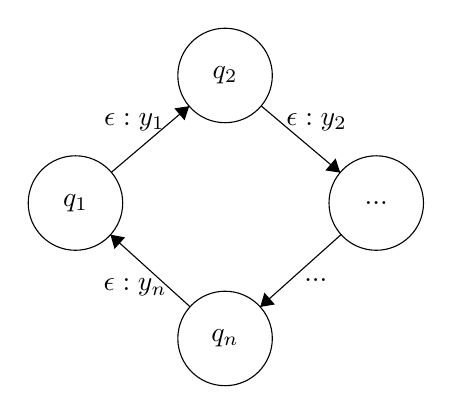
\begin{tikzpicture}[scale=0.2]
 	\tikzstyle{every node}+=[inner sep=0pt]
 	\draw [black] (12.8,-13.3) circle (3);
 	\draw (12.8,-13.3) node {$q_1$};
 	\draw [black] (22.3,-5.2) circle (3);
 	\draw (22.3,-5.2) node {$q_2$};
 	\draw [black] (31.9,-13.3) circle (3);
 	\draw (31.9,-13.3) node {$...$};
 	\draw [black] (22.3,-21.9) circle (3);
 	\draw (22.3,-21.9) node {$q_n$};
 	\draw [black] (15.08,-11.35) -- (20.02,-7.15);
 	\fill [black] (20.02,-7.15) -- (19.08,-7.29) -- (19.73,-8.05);
 	\draw (16.54,-8.76) node [above] {$\epsilon:y_1$};
 	\draw [black] (24.59,-7.13) -- (29.61,-11.37);
 	\fill [black] (29.61,-11.37) -- (29.32,-10.47) -- (28.67,-11.23);
 	\draw (28.11,-8.76) node [above] {$\epsilon:y_2$};
 	\draw [black] (29.67,-15.3) -- (24.53,-19.9);
 	\fill [black] (24.53,-19.9) -- (25.46,-19.74) -- (24.8,-18.99);
 	\draw (28.06,-18.09) node [below] {$...$};
 	\draw [black] (20.08,-19.89) -- (15.02,-15.31);
 	\fill [black] (15.02,-15.31) -- (15.28,-16.22) -- (15.95,-15.48);
 	\draw (16.59,-18.09) node [below] {$\epsilon:y_n$};
 	\end{tikzpicture}
 \end{center}
 Any non-deterministic model of Mealy automaton that doesn't allow $\epsilon$ cycles will have less expressive power.
 
 One example of such model where cycles become illegal is class $ \mathbb{M} \cap \mathcal{P}(\Sigma^* \rightarrow \Gamma^*)$. The only cases when cycles are ok, is when after reaching any of states $q_1$,..$q_n$ it's impossible to accept. But in such case we might as well delete the whole thing as those states are redundant. Another special case is when $y_1=\epsilon$,...$y_n=\epsilon$, but then again we might simplify it by removing $\epsilon:\epsilon$ edges in a way analogical to removing $\epsilon$ edges in NFA. Therefore such cycles are either not allowed , redundant or erasable. Thanks to $\epsilon$-cycles being illegal, we can in fact reduce \underline{almost} every $\epsilon$-Mealy-automaton to $\epsilon$-free one. This:
 
 \begin{center}
 	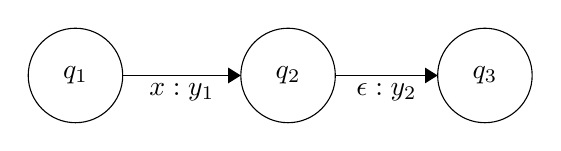
\begin{tikzpicture}[scale=0.2]
 	\tikzstyle{every node}+=[inner sep=0pt]
 	\draw [black] (18.2,-13.2) circle (3);
 	\draw (18.2,-13.2) node {$q_2$};
 	\draw [black] (30.7,-13.2) circle (3);
 	\draw (30.7,-13.2) node {$q_3$};
 	\draw [black] (4.7,-13.2) circle (3);
 	\draw (4.7,-13.2) node {$q_1$};
 	\draw [black] (21.2,-13.2) -- (27.7,-13.2);
 	\fill [black] (27.7,-13.2) -- (26.9,-12.7) -- (26.9,-13.7);
 	\draw (24.45,-13.7) node [below] {$\epsilon:y_2$};
 	\draw [black] (7.7,-13.2) -- (15.2,-13.2);
 	\fill [black] (15.2,-13.2) -- (14.4,-12.7) -- (14.4,-13.7);
 	\draw (11.45,-13.7) node [below] {$x:y_1$};
 	\end{tikzpicture}
 \end{center}
 should become this:
 \begin{center}
 	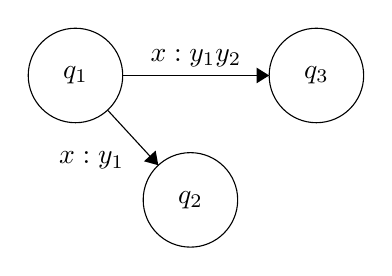
\begin{tikzpicture}[scale=0.2]
 	\tikzstyle{every node}+=[inner sep=0pt]
 	\draw [black] (11.9,-6.4) circle (3);
 	\draw (11.9,-6.4) node {$q_1$};
 	\draw [black] (27.2,-6.4) circle (3);
 	\draw (27.2,-6.4) node {$q_3$};
 	\draw [black] (19.2,-14.3) circle (3);
 	\draw (19.2,-14.3) node {$q_2$};
 	\draw [black] (14.9,-6.4) -- (24.2,-6.4);
 	\fill [black] (24.2,-6.4) -- (23.4,-5.9) -- (23.4,-6.9);
 	\draw (19.55,-5.9) node [above] {$x:y_1y_2$};
 	\draw [black] (13.94,-8.6) -- (17.16,-12.1);
 	\fill [black] (17.16,-12.1) -- (16.99,-11.17) -- (16.25,-11.85);
 	\draw (15.02,-11.81) node [left] {$x:y_1$};
 	\end{tikzpicture}
 \end{center}
 The only $\epsilon$ that could not be erased this way are those that go straight out of initial state $q_0$. Some of them can be erased by replacing this:
 
 \begin{center}
 	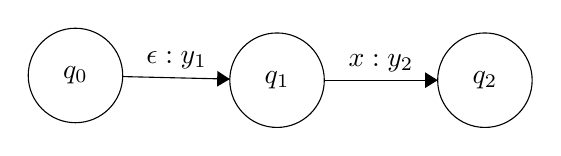
\begin{tikzpicture}[scale=0.2]
 	\tikzstyle{every node}+=[inner sep=0pt]
 	\draw [black] (11.9,-6.4) circle (3);
 	\draw (11.9,-6.4) node {$q_0$};
 	\draw [black] (24.7,-6.7) circle (3);
 	\draw (24.7,-6.7) node {$q_1$};
 	\draw [black] (37.9,-6.7) circle (3);
 	\draw (37.9,-6.7) node {$q_2$};
 	\draw [black] (14.9,-6.47) -- (21.7,-6.63);
 	\fill [black] (21.7,-6.63) -- (20.91,-6.11) -- (20.89,-7.11);
 	\draw (18.32,-6) node [above] {$\epsilon:y_1$};
 	\draw [black] (27.7,-6.7) -- (34.9,-6.7);
 	\fill [black] (34.9,-6.7) -- (34.1,-6.2) -- (34.1,-7.2);
 	\draw (31.3,-6.2) node [above] {$x:y_2$};
 	\end{tikzpicture}
 \end{center}
 with this:
 
 \begin{center}
 	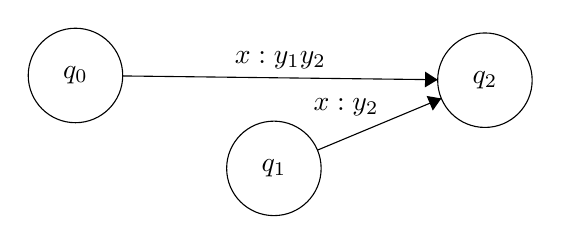
\begin{tikzpicture}[scale=0.2]
 	\tikzstyle{every node}+=[inner sep=0pt]
 	\draw [black] (11.9,-6.4) circle (3);
 	\draw (11.9,-6.4) node {$q_0$};
 	\draw [black] (24.5,-12.3) circle (3);
 	\draw (24.5,-12.3) node {$q_1$};
 	\draw [black] (37.9,-6.7) circle (3);
 	\draw (37.9,-6.7) node {$q_2$};
 	\draw [black] (27.27,-11.14) -- (35.13,-7.86);
 	\fill [black] (35.13,-7.86) -- (34.2,-7.7) -- (34.59,-8.63);
 	\draw (29.08,-8.97) node [above] {$x:y_2$};
 	\draw [black] (14.9,-6.43) -- (34.9,-6.67);
 	\fill [black] (34.9,-6.67) -- (34.11,-6.16) -- (34.09,-7.16);
 	\draw (24.91,-6.01) node [above] {$x:y_1y_2$};
 	\end{tikzpicture}
 \end{center}
 
 However if state $q_2$ is accepting, then the epsilon transition expresses mapping $M(\epsilon,k)$ such that $k\ne\epsilon$. We cannot get rid of it completely. This shows another place where $\epsilon$ strictly increases expressive power. For this reason defining non-deterministic Mealy automata as $\delta : Q \times \Sigma \rightarrow \mathcal{P}(Q,\Gamma^*)$ grants them inherently less power.
 
 Another place where epsilons change a lot is the difference between $\delta : Q \times (\Sigma \cup \{\epsilon\}) \rightarrow \mathcal{P}(Q,\Gamma)$ and $\delta : Q \times \Sigma  \rightarrow \mathcal{P}(Q,\Gamma)$. You can  simulate multi-output $\Gamma^*$:
 \begin{center}
 	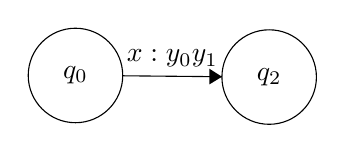
\begin{tikzpicture}[scale=0.2]
 	\tikzstyle{every node}+=[inner sep=0pt]
 	\draw [black] (11.9,-6.4) circle (3);
 	\draw (11.9,-6.4) node {$q_0$};
 	\draw [black] (24.2,-6.5) circle (3);
 	\draw (24.2,-6.5) node {$q_2$};
 	\draw [black] (14.9,-6.42) -- (21.2,-6.48);
 	\fill [black] (21.2,-6.48) -- (20.4,-5.97) -- (20.4,-6.97);
 	\draw (18.05,-5.92) node [above] {$x:y_0y_1$};
 	\end{tikzpicture}
 \end{center}
 using epsilons like this:
 \begin{center}
 	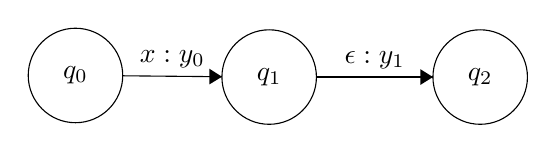
\begin{tikzpicture}[scale=0.2]
 	\tikzstyle{every node}+=[inner sep=0pt]
 	\draw [black] (11.9,-6.4) circle (3);
 	\draw (11.9,-6.4) node {$q_0$};
 	\draw [black] (24.2,-6.5) circle (3);
 	\draw (24.2,-6.5) node {$q_1$};
 	\draw [black] (37.6,-6.5) circle (3);
 	\draw (37.6,-6.5) node {$q_2$};
 	\draw [black] (14.9,-6.42) -- (21.2,-6.48);
 	\fill [black] (21.2,-6.48) -- (20.4,-5.97) -- (20.4,-6.97);
 	\draw (18.05,-5.93) node [above] {$x:y_0$};
 	\draw [black] (27.2,-6.5) -- (34.6,-6.5);
 	\fill [black] (34.6,-6.5) -- (33.8,-6) -- (33.8,-7);
 	\draw (30.9,-6) node [above] {$\epsilon:y_1$};
 	\end{tikzpicture}
 \end{center}
 where $y_0,y_1\in\Gamma$. Without epsilons, multi-output strictly increases power.
 
 We can also use epsilons to simulate duplicate input labels. Every structure of this form:
 \begin{center}
 	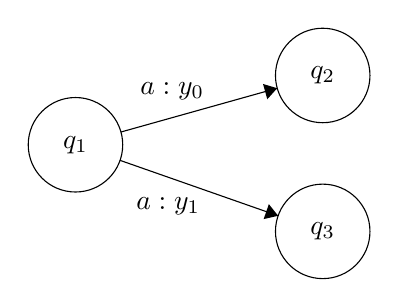
\begin{tikzpicture}[scale=0.2]
 	\tikzstyle{every node}+=[inner sep=0pt]
 	\draw [black] (11.4,-10.3) circle (3);
 	\draw (11.4,-10.3) node {$q_1$};
 	\draw [black] (27.1,-5.9) circle (3);
 	\draw (27.1,-5.9) node {$q_2$};
 	\draw [black] (27.1,-15.8) circle (3);
 	\draw (27.1,-15.8) node {$q_3$};
 	\draw [black] (14.29,-9.49) -- (24.21,-6.71);
 	\fill [black] (24.21,-6.71) -- (23.31,-6.44) -- (23.58,-7.41);
 	\draw (17.54,-7.48) node [above] {$a:y_0$};
 	\draw [black] (14.23,-11.29) -- (24.27,-14.81);
 	\fill [black] (24.27,-14.81) -- (23.68,-14.07) -- (23.35,-15.02);
 	\draw (17.29,-13.62) node [below] {$a:y_1$};
 	\end{tikzpicture}
 \end{center}
 would be rewritten as:
 \begin{center}
 	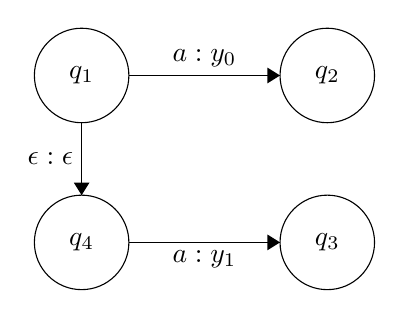
\begin{tikzpicture}[scale=0.2]
 	\tikzstyle{every node}+=[inner sep=0pt]
 	\draw [black] (11.5,-5.9) circle (3);
 	\draw (11.5,-5.9) node {$q_1$};
 	\draw [black] (27.1,-5.9) circle (3);
 	\draw (27.1,-5.9) node {$q_2$};
 	\draw [black] (27.1,-16.5) circle (3);
 	\draw (27.1,-16.5) node {$q_3$};
 	\draw [black] (11.5,-16.5) circle (3);
 	\draw (11.5,-16.5) node {$q_4$};
 	\draw [black] (14.5,-5.9) -- (24.1,-5.9);
 	\fill [black] (24.1,-5.9) -- (23.3,-5.4) -- (23.3,-6.4);
 	\draw (19.3,-5.4) node [above] {$a:y_0$};
 	\draw [black] (11.5,-8.9) -- (11.5,-13.5);
 	\fill [black] (11.5,-13.5) -- (12,-12.7) -- (11,-12.7);
 	\draw (11,-11.2) node [left] {$\epsilon:\epsilon$};
 	\draw [black] (14.5,-16.5) -- (24.1,-16.5);
 	\fill [black] (24.1,-16.5) -- (23.3,-16) -- (23.3,-17);
 	\draw (19.3,-17) node [below] {$a:y_1$};
 	\end{tikzpicture}
 \end{center}
 
 You can summarize the hierarchy of power as:
 \begin{enumerate}
 	\item Most powerful is $\delta : Q \times (\Sigma \cup \{\epsilon\})\rightarrow \mathcal{P}(Q \times  (\Gamma \cup \{\epsilon\}))$ and it's equivalent to $\delta : Q \times  (\Sigma \cup \{\epsilon\}) \rightarrow \mathcal{P}(Q \times \Gamma^*)$ and $\delta : Q \times  (\Sigma \cup \{\epsilon\}) \rightarrow Q \times \Gamma^*$ and $\delta : Q \times  (\Sigma \cup \{\epsilon\}) \rightarrow Q \times (\Gamma\cup\{\epsilon \})$
 	\item Then there is $\delta : Q \times (\Sigma \cup \{\epsilon\})\rightarrow \mathcal{P}(Q \times  (\Gamma \cup \{\epsilon\}))$ without epsilon cycles, which is equivalent to $\delta : Q \times (\Sigma \cup \{\epsilon\})\rightarrow \mathcal{P}(Q \times  \Gamma^*)$ without epsilon cycles.
 	\item Then $\delta : Q \times \Sigma \rightarrow \mathcal{P}(Q \times \Gamma^*)$
 	\item Then $\delta : Q \times \Sigma \rightarrow \mathcal{P}(Q \times  (\Gamma \cup \{\epsilon\}))$
 	\item Then $\delta : Q \times \Sigma \rightarrow \mathcal{P}(Q \times  \Gamma)$
 \end{enumerate}
 
\section{Hierarchy of classes} Obviously $\mathbb{M}_0 \subsetneq \mathbb{M}_{\infty}  \subsetneq \mathbb{ M}_\vee \subsetneq \mathbb{M}_{\rightarrow}  \subsetneq \mathbb{M} $, but now when we have all the necessary tools and definitions we  can show further the correlations between Mealy machine models and classes of relations and their encodings:
 \begin{enumerate}


\item $\mathbb{S}(\mathbb{M}) \subset \mathbb{CFG}$ Class of relations generated by non-deterministic Mealy machines is a proper subclass of context-free separated relations. The proof idea is simple: \\
Given non-deterministic Mealy automaton $M$ on alphabets $\Sigma$ and $\Gamma$ we build context-free grammar with non-terminal alphabet $V$ and terminal alphabet $\Sigma \cup \Gamma \cup \{\#\}$. For any $(q,s,q') \in \delta \subset Q \times (\Sigma \cup \{\epsilon\}) \rightarrow Q$ and $(q,s,s') \in G \subset Q \times (\Sigma \cup \{\epsilon\}) \rightarrow (\Gamma \cup \{\epsilon\})$ we generate context-free rule $V_q \rightarrow s V_{q'} s'$.  We also add initial rule $S \rightarrow V_{q_0}$ where $q_0$ is initial state of $M$. At the end for every $q \in F$ we add rules $V_q \rightarrow \#$. If for any given string $w \in \Sigma \cup \Gamma \cup \{\#\}$ there exists a valid derivation tree in such CFG, then we can be sure that there exists a corresponding path in $M$ that leads from initial to final state and produces $w$ along the way. \\
Unfortunately it's not true that any context-free relation can be generated by Mealy machines (the proof is quite obvious). $ \mathbb{CFG} \not\subset \mathbb{S}(\mathbb{M})$

\item $\mathbb{REG} \cap \mathbb{S}(\mathbb{M}) \subsetneq \mathbb{S}(\mathbb{M})$ Class of relations generated by non-deterministic Mealy machines is a proper superclass of regular separated relations. We need to prove that $\mathbb{REG} \cap \mathbb{S}(\mathbb{M}) \subset \mathbb{S}(\mathbb{M})$ and $\mathbb{S}(\mathbb{M}) \not\subset \mathbb{REG} \cap \mathbb{S}(\mathbb{M})$. The first case is trivial. The second is much more tedious. Here is its proof: \\
Assume to the contrary that for any $M \in \mathbb{M}$, we can find finite state automaton $P$ that recognizes  $\mathbb{S}(M)$. Let's take the first projection of $\mathbb{S}(M)$ given by 
$\Pi_0 = \{s \in \Sigma^* : \exists_{t\in\Gamma^*} s\#t \in M\}$. We can always find such automaton $P'$ that is a sub-automaton of $P$ (has some states and edges removed, no new edges or states are added, and additionally accepting states can be changed) and accepts $\Pi_0$. Because every string $s \in  \mathbb{S}(M)$ must contain exactly one $\#$, we can deduce that once $P'$ accepts, some transition labeled with $\#$ must take you to some new state such that: 1. it is in $P$ , 2. it is not in $P'$ , 3. it's not possible to ever go back to any state in $P'$, 4. it is possible to  reach accepting state of $P$. We will call such states the $\#$-states, and their edges that connect $P$ with $P'$ are the $\#$-edges (those edges don't belong to $P'$). Notice that there can only be finitely many such $\#$-states and each of them has exactly one $\#$-edge. We can divide $\Pi_0$ into congruence classes based on which accepting state in $P'$ they end up in (and which $\#$-edge they transition through). The most important implication that follows from it is that we can also divide $ \mathbb{S}(M)$ based on this criterion - given $(s_0,t_0),(s_1,t_1) \in \mathbb{S}(M)$ the two relations are congruent iff $s_0$ and $s_1$ are congruent too. Because $P'$ has only finitely many accepting states, there can be only finitely many congruence classes. The property of such congruence is that if $(s_0,t_0)$ is congruent with $(s_1,t_1)$ then $(s_0,t_1),(s_1,t_0)\in M$ (because both $s_0$ and $s_1$ reached the same $\#$-state and both $s_0\#$ and $s_1\#$ transitioned over the same $\#$-edge, so at that point the automaton lost all memory about whether the left-side element of pair was $s_0$ or $s_1$ and it will have to behave the same way in both cases and accept the same right-side elements of pair). Obviously this property does not hold for all non-deterministic Mealy automata in general. They might require infinitely many congruence classes to make such property hold.

\item $\mathbb{REG} \cap \mathbb{S}(\mathbb{M}) \not\subset \mathbb{S}(\mathbb{M}_\vee)$  This one is quite obvious. $\mathbb{S}(\mathbb{M}_\vee)$ only contains relations that are  functions while $\mathbb{REG} \cap \mathbb{S}(\mathbb{M})$ contains any relations.  

\item $\mathbb{S}(\mathbb{M}_\vee)\not\subset\mathbb{REG} \cap\mathbb{S}(\mathbb{M})$ To prove this one we can reuse proof of $\mathbb{REG} \cap \mathbb{S}(\mathbb{M}) \subsetneq \mathbb{S}(\mathbb{M})$. Every finite state automaton from class of regular separated relations $\mathbb{REG} \cap \mathbb{S}(\mathbb{M})$ contains finitely many $\#$-states. However, look at this counter-example of $M \in \mathbb{M}_\vee$ given by: \\
$M(x) = \begin{cases}
0^{\vert x \vert} & \mbox{if }  x  \in 1^*   \\
\mbox{reject} & \mbox{otherwise} 
\end{cases}$ \\
There are infinitely many relations of form $(1^n,0^n)$  generated by $M$ and for none of them it holds that if $(1^n,0^n)$ is congruent with $(1^m,y^m)$ then $(1^n,0^m), (1^m,y^n)  \in M$. This leads to contradiction.


\item $\mathbb{REG} = \mathbb{I}(\mathbb{M})$  Class of relations generated by non-deterministic Mealy machines is exactly equal to class of regular interleaved relations. 

First we prove $\mathbb{I}(\mathbb{M})  \subset \mathbb{REG} $. The proof is constructive and the idea is simple - you just "flatten" input and output together. Let $M \in \mathbb{M}$ be non-determinisitc Mealy relation in $\Sigma^* \times \Gamma^*$ such that $\Sigma \cap \Gamma = \emptyset$. We will build a finite state automaton $P \subset (\Sigma \cup \Gamma)^*$ such that its recognized language is equivalent to one of possible interleaved encodings $ P = \mathbb{I}(M)$ . For every state $m \in Q_M$ and alphabet character $s \in \Sigma \cup \{\epsilon\}$ there is transition $m' = \delta_M(m,s)$ and output $s' = G_M(m,s) \in \Gamma \cup \{\epsilon\}$. Then in $P$ there shall exist $(p_m,s,p_{ms}), (p_{ms},s',p_{m'}) \in \delta_P \subset Q_P \times (\Sigma \cup \Gamma \cup \{\epsilon\}) \rightarrow Q_P$. So for every transition in $\delta_M$ and output in $G_M$ there is corresponding state in $Q_P$ that simulates it. First $P$ reads some input $\Sigma$ then goes to a new state that expects to read output $\Gamma$. Such construction implements a particular encoding of $\mathbb{I}(M)$ - such that exactly corresponds to order of reading and printing events in $M$. To finalize this construction we need to specify that for every accepting state $m \in F_M$ there is a corresponding accepting state $p_m$ and for initial state $m_0$ there is also initial state $p_{m_0}$. 
 
 Now we prove $\mathbb{REG} \subset \mathbb{I}(\mathbb{M})$ . Suppose $P$ is some deterministic finite automaton over alphabet $\Sigma$. We can always split $\Sigma$ into $\Sigma_0$ and $\Sigma_1$ such that $\Sigma_0 \cap \Sigma_1 = \emptyset$ and $\Sigma_0 \cup \Sigma_1 = \Sigma$. Every string in $\Sigma$ becomes at the same time also some interleaved pair in $\Sigma_0 \times \Sigma_1$. We attempt to build non-deterministic Mealy machine $M$ that accepts every such pair, except that this time for convenience (as both models are equivalent) we define transition function as $\delta_M : Q_M \times \Sigma \cup \{\epsilon\} \rightarrow \mathcal{P}(Q_M \times \Gamma)$ without output function $G$ (output is encoded in $\delta$ instead).  For every $(p,s,p') \in \delta_P \subset Q_P \times \Sigma \rightarrow Q_P$ there are 2 possibilities: 
\begin{enumerate}
	\item if $s \in \Sigma_0$ then put $(m_{p'},\epsilon) \in \delta_M(m_p,s) $ 
	\item if $s \in \Sigma_1$ then put $(m_{p'},s) \in \delta_M(m_p,\epsilon) $ 
\end{enumerate}
For every state $p \in F_P$ put $m_p \in F_M$. Finally let $m_{p_0}$ be the accepting state. This ends construction of such $M$  that exactly simulates $\mathbb{I}(M) = P$.

\item $\mathbb{I}(\mathbb{M}_\vee) \subset \mathbb{REG}$ This one is very simple to show and proof is analogous to the proof of $\mathbb{I}(\mathbb{M}) \subset \mathbb{REG}$. First you need to consider that any $M \in \mathbb{M}_\vee$ is equivalent to union of several $M_t \in\mathbb{M}_\infty$ (one for each tape $t \in T$). Any automaton in $\mathbb{M}_\infty$ can be treated as a specific case of non-deterministic automaton $\mathbb{M}$, that just happens to lack non-determinism. Therefore we already know that for each $t\in T$ we have $\mathbb{I}(M_t) \subset \mathbb{REG}$. We can also be sure that regular languages are closed under union which gives us $\mathbb{I}(M_{t_0}) \cup \mathbb{I}(M_{t_1}) \cup ... = \mathbb{I}(M) \subset \mathbb{REG}$ (we simulate very tape separately but we also have guarantee that only one of them accepts at the time therefore this equality holds). Unfortunately the opposite is not true $\mathbb{REG} \not\subset \mathbb{I}(\mathbb{M}_\vee) $ because $\mathbb{M}_\vee$ require determinism.

\item $\mathbb{M}_\vee \cap \mathcal{P}(\Sigma^* \times \Gamma^*) \subsetneq  \mathbb{M} \cap \mathcal{P}(\Sigma^* \rightarrow \Gamma^*)$ If we remove from class of non-deterministic Mealy machines, all those instances that produce multiple outputs simultaneously, and keep only those machines that correspond to functions on languages, then the obtained class is still larger than class decidable by disjunctive Mealy machines. The implication $\mathbb{M}_\vee \cap \mathcal{P}(\Sigma^* \times \Gamma^*) \subset  \mathbb{M} \cap \mathcal{P}(\Sigma^* \rightarrow \Gamma^*)$ is trivial. You just non-deterministically simulate all the tapes at the same time. The inequality can be proved with simple counterexample:
\begin{center}
	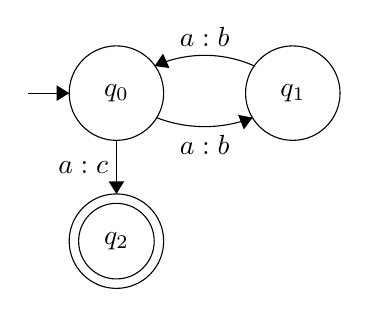
\begin{tikzpicture}[scale=0.2]
	\tikzstyle{every node}+=[inner sep=0pt]
	\draw [black] (12.8,-9.5) circle (3);
	\draw (12.8,-9.5) node {$q_0$};
	\draw [black] (24,-9.5) circle (3);
	\draw (24,-9.5) node {$q_1$};
	\draw [black] (12.8,-18.9) circle (3);
	\draw (12.8,-18.9) node {$q_2$};
	\draw [black] (12.8,-18.9) circle (2.4);
	\draw [black] (7.2,-9.5) -- (9.8,-9.5);
	\fill [black] (9.8,-9.5) -- (9,-9) -- (9,-10);
	\draw [black] (21.454,-11.056) arc (-68.75856:-111.24144:8.429);
	\fill [black] (21.45,-11.06) -- (20.53,-10.88) -- (20.89,-11.81);
	\draw (18.4,-12.13) node [below] {$a:b$};
	\draw [black] (12.8,-12.5) -- (12.8,-15.9);
	\fill [black] (12.8,-15.9) -- (13.3,-15.1) -- (12.3,-15.1);
	\draw (12.3,-14.2) node [left] {$a:c$};
	\draw [black] (15.233,-7.778) arc (114.17742:65.82258:7.732);
	\fill [black] (15.23,-7.78) -- (16.17,-7.91) -- (15.76,-6.99);
	\draw (18.4,-6.6) node [above] {$a:b$};
	\end{tikzpicture}
\end{center}
This automaton decides relation: \\
a:c \\
aaa:bbc \\
aaaaa:bbbbc \\
and so on..\\
Notice that for any two accepted pairs, the rule of common prefixes doesn't hold. However, in case of $\mathbb{ M}_\vee$ automata, the prefix rule must hold within each tape. Therefore any $M \in \mathbb{ M}_\vee$ can be partitioned  into finite number of equivalence classes induced by the prefix rule. This counter-example shows that there exists automaton in $\mathbb{ M}_\vee$ that describes a function but still requires infinite number of such equivalence classes.


\item $\mathbb{M}_\rightarrow \cap \mathcal{P}(\Sigma^* \times \Gamma^*) =  \mathbb{M} \cap \mathcal{P}(\Sigma^* \rightarrow \Gamma^*)$ If we remove from class of non-deterministic Mealy machines, all those instances that produce multiple outputs simultaneously, and keep only those machines that correspond to functions on languages, then the obtained class is equal to class of functional Mealy machines. First let's prove  $\mathbb{M} \cap \mathcal{P}(\Sigma^* \rightarrow \Gamma^*) \subset \mathbb{M}_\rightarrow \cap \mathcal{P}(\Sigma^* \times \Gamma^*)   $.

 Define computation context $\gamma$ to be set of states and all their currently associated outputs (so it's relation $\gamma \subset Q \times \Gamma^*$). We should write $\gamma_x(q) = \{s_0,s_1,...\}$ to denote that after reading $x\in\Sigma^*$, at state $q$ there will be strings $s_0,s_1,...\in\Gamma^*$ produced so far in current non-deterministic computation branch. Here is an example:
\begin{center}
\begin{table}[!htbp]
	\renewcommand\arraystretch{1.5}
	\centering
	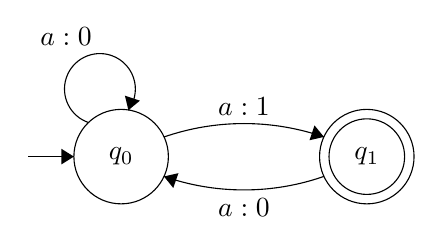
\begin{tikzpicture}[baseline=(current bounding box.center),scale=0.2]
	\tikzstyle{every node}+=[inner sep=0pt]
	\draw [black] (24.6,-13.2) circle (3);
	\draw (24.6,-13.2) node {$q_1$};
	\draw [black] (24.6,-13.2) circle (2.4);
	\draw [black] (9,-13.2) circle (3);
	\draw (9,-13.2) node {$q_0$};
	\draw [black] (11.723,-11.953) arc (109.07296:70.92704:15.536);
	\fill [black] (21.88,-11.95) -- (21.28,-11.22) -- (20.96,-12.16);
	\draw (16.8,-10.6) node [above] {$a:1$};
	\draw [black] (3.1,-13.2) -- (6,-13.2);
	\fill [black] (6,-13.2) -- (5.2,-12.7) -- (5.2,-13.7);
	\draw [black] (6.936,-11.039) arc (251.4189:-36.5811:2.25);
	\draw (5.5,-6.18) node [above] {$a:0$};
	\fill [black] (9.46,-10.25) -- (10.19,-9.65) -- (9.24,-9.33);
	\draw [black] (21.881,-14.456) arc (-70.78185:-109.21815:15.435);
	\fill [black] (11.72,-14.46) -- (12.31,-15.19) -- (12.64,-14.25);
	\draw (16.8,-15.82) node [below] {$a:0$};
	\end{tikzpicture}\hspace{5mm}
	\begin{tabular}{|l|l|l|l|}
		\hline
		$\gamma$          & $q_0$      & $q_1$       \\ \hline
		$\gamma_\epsilon$ & $\epsilon$ & $\emptyset$                 \\ \hline
		$\gamma_a$        &      $0$      &      $1$                     \\ \hline
		$\gamma_{aa}$     &     $00,10$       &         $01$           \\ \hline
		$\gamma_{aaa}$    &       $000,100,010$     &  $001,101$                        \\ \hline
	\end{tabular}
\end{table}

\end{center}


Notice that automaton is a function $\Sigma^* \rightarrow \Gamma^*$, iff $\forall_{x\in\Sigma^*} \forall_{q\in F} \vert \gamma_x(q) \vert \le 1$. We should also define reachability $\phi \subset Q \times Q$ of each state $q\in Q$ as set of states $\phi(q) = \{q_k,q_l,q_m,...\}$ such that all states $q_k,q_l,q_m,...$ can be reached from $q$. In the example above, the reachability is given by: \\
$\phi(q_0) = \{q_0,q_1\}$ \\
$\phi(q_1) = \{q_0,q_1\}$ \\
Of course is holds that if $\vert \gamma_s(q) \vert = n$ and $q' \in \phi(q)$ then $\vert \gamma_{s'}(q') \vert \ge n$ where $s$ is prefix of $s'$ and $s'$ leads to $q'$. That's because: \\
$\forall_{q,q'\in Q} \forall_{s\in\Sigma} \forall_{s' \in \Gamma^*} (q',s') \in \delta(q,s) \implies  \gamma(q)s' \subset \gamma_{s}(q')$  \\
and if $\{s_0,s_1\} \subset\gamma(q)$ then $\{s_0s',s_1s'\} \subset\gamma_s(q')$ where of course $s_0 \ne s_1 \implies s_0s' \ne s_1s'$. Due to modus tollens we derive: \\ 
$\forall_{x\in\Sigma^*} \forall_{q\in F} \vert \gamma_x(q) \vert \le 1$ and \\
$\vert \gamma_s(q) \vert > 1 \implies \vert \gamma_{s'}(q') \vert  > 1$ then \\ $\forall_{x\in\Sigma^*} \forall_{q\in Q} \phi(q) \cap F \ne \emptyset \implies  \vert \gamma_x(q) \vert \le 1$ \\
And in case of non-deterministic automata we can without any worries remove all such states that $ \phi(q) \cap F = \emptyset$, therefore we are left with: \\
$\forall_{x\in\Sigma^*} \forall_{q\in Q} \vert \gamma_x(q) \vert \le 1$ \\
This give us very strong guarantees but there is one more property automaton must satisfy in order to express functions.


At any given point $x \in \Sigma^*$ in computation context, there could be at most one accepting state with $\gamma_x \ne \emptyset$. This could be written as: \\
$\forall_{x\in\Sigma^*} \vert \bigcup_{q\in F} \gamma_x(q) \vert \le 1$ \\
Therefore let's consider $\psi : \Sigma^* \rightarrow \mathcal{P}(Q)$ to be a function that returns all non-empty states at any given time in computation context: \\
$\psi(x) = \{q \in Q : \gamma_x(q) \ne \emptyset \}$ \\
Initially automaton starts with $\psi(\epsilon)$ and then it must inductively guarantee that: \\
$\vert \psi(x) \cap F \vert \le 1 \implies  \forall_{s\in\Sigma}  \vert \psi(xs) \cap F \vert \le 1$ \\
Let's denote by $Q_\psi$ set of all context states reachable in such way: \\
$Q_\psi = \{ q \in \mathcal{P}(Q) : \exists_{x\in\Sigma^*} \psi(x)=q \}$ \\
Moreover we can compose elements of $q \in Q_\psi$ with strings $s\in\Sigma$. Such composition should yield the next elements of $Q_\psi$ that the automaton would transition to: \\
$qs = q' \iff   \exists_{x\in\Sigma^*} \psi(x)=q \wedge \psi(xs)=q' $  \\
Notice that the $x$ can be arbitrary, because we only care whether $\gamma_x(q)$ is $\emptyset$ or not. The exact contents don't matter, therefore all sequences that lead to $q$ are equivalent.


Thanks to $\forall_{x\in\Sigma^*} \forall_{q\in Q} \vert \gamma_x(q) \vert \le 1$ we can also show special property of how $\delta$ behaves with $Q_\psi$. Let's say that $q_1,q_2 \in  \psi(x)$, $s \in \Sigma$ and $(q',s_1') \in \check{\delta}(q_1,s)$ and $(q',s_2') \in \check{\delta}(q_2,s)$ (where $\check{\delta} : Q \times \Sigma \rightarrow \mathcal{P}(Q \times \Gamma^*)$ stands for extended version of $\delta$ that additionally follows  $\epsilon$ transitions). This means that both $\gamma_x(q_1)s_1' \in \gamma_{xs}(q') $ and $\gamma_x(q_2)s_2' \in \gamma_{xs}(q') $, but because we guarantee that $\vert \gamma_{xs}(q')\vert \le 1$ we can conclude that $\gamma_x(q_2)s_2' = \gamma_x(q_1)s_1'$. So in other words, every time two non-deterministic branches transition into the same state $q'$, they must carry the same output string.

 We can now use it to determinize automaton from $M\in\mathbb{M}$ to some $N\in\mathbb{M}_\rightarrow$. The procedure looks very similar to turning NFA to FSA. (Of course we assume $\delta_M : Q \times (\Gamma \cup \{\epsilon \}) \rightarrow Q \times \Gamma^*$ ).
Construction of $N$ looks like this:\\
$Q_N = Q_\psi \subset \mathcal{P}(Q_M) $ \\
$T_N = Q_M $ \\
$\delta_N(q_n,s) = q_n s $ where $q_n\in Q_N$ is at the same time a set $q_n \subset Q_M$ and element $q_n \in Q_\psi $, therefore concatenation $q_ns \in Q_\psi = Q_N$\\
$G_N(q,s,t') = (s',t) \iff t \in q \subset  Q_M \wedge t' \in \delta_N(q,s) \subset  Q_M \wedge (t',s') \in \check{\delta}_M(t,s) $ where we have the guarantee that either there is only one $t$ that leads  to $t'$ by following $(t',s') \in \check{\delta}_M(t,s)$ or there are multiple possible $t$ but we can chose arbitrary of them because all the transitions must produce the same output (as explained above).\\
$F_N(q_n) = q_n \cap F_M$ is guaranteed to be either empty or singleton. \\
$q_{0N} = \psi(\epsilon)$ \\
And of course notice the correspondence between $\gamma_x(q)$ of $M$ and $\gamma(x,q)$ of $N$. This gives you initial state of memory cells as: \\
$\gamma(q_{0N},\epsilon,t) = \gamma_\epsilon(t)$ \\

This ends the construction of $N$. Moreover it's easy to follow it in reverse order (there is 1-to-1 correspondence between most of the elements, and in places where the correspondence is one-to-many the choice can be made arbitrarily as it was in case of $t$ such that $(t',s') \in \check{\delta}_M(t,s)$). Nonetheless it's easy to show that converse $\mathbb{M}_\rightarrow \cap \mathcal{P}(\Sigma^* \times \Gamma^*) \subset   \mathbb{M} \cap \mathcal{P}(\Sigma^* \rightarrow \Gamma^*) $ holds as well.



\end{enumerate}


\subparagraph{End-of-string markers} Disjunctive Mealy machines come with one of determinism's inherent problems. They can't non-deterministically check for end of input. We need to add special marker at the end to facilitate it. Such marker  actually extends expressive power. Without it determinisitc Mealy machines cannot relate any output to empty string (because in case of empty string, no transition is ever made and no output is ever produced). We could achieve similar effect by adding special marker at the beginning instead. Both beginning and end markers extend power of automaton however, end  marker gives more power than beginning marker. With just the beginning marker you can express $M(\epsilon,0)$ but you cannot express $M(x) = x0$ (where $M \subset \{0\}^* \rightarrow \{0\}^*$), whilst both can be expressed with end marker. On top of that you can notice a striking connection between end-of-string marker and $\#$ separator of $\mathbb{S}$ encoding. Indeed these two have a lot in common. For this reason we will also use $\#$ to denote end-of-string marker. Of course the $\#$ should not be actually treated as part  of formal language. We will slightly change the definition in this case to:


let $M\subset \Sigma^* \rightarrow \Gamma^*$ then $\forall_{x\in \Sigma^*,y\in\Gamma^*} M(x,y) \iff M$ returns $y$ on input $x\#$. Transition function of $M$ is $\delta : Q \times (\Sigma \cup \{\#\}) \rightarrow Q$. Output function is $G : Q \times (\Sigma \cup \{\#\}) \times T \rightarrow \Gamma^*$. Of course it must also hold that $\# \notin \Sigma$. We will denote class of such automata as $\mathbb{M}_{\#\vee}$.

Notice that given $M \in \mathbb{M}_\vee$ and $M_\# \in \mathbb{M}_{\#\vee}$ such that $M \in \Sigma^*\# \rightarrow \Gamma^*$ and $M_\# \in \Sigma^* \rightarrow \Gamma^*$ there exists an isomorphism $f : \Sigma^* \rightarrow \Sigma^*\#$ such that $M(f(x)) = M_\#(x)$. You can treat it as $M \circ f \rightsquigarrow M_\#$. Notice that function $f$ can by itself be treated as relation on languages where $\Sigma$ is input alphabet and $\Sigma\cup\{\#\}$ is output. Let $\#$ be some kind of Mealy automaton that implements $f$. Then composition of automata yields $M\# = M_\#$. Such composition forms a semigroup of language relations. Also, since $f$ is a bijection we can find an inverse element $\#^{-1}$ that works the opposite way:  $M = M\#\#^{-1} = M_\#\#^{-1}$.


\subparagraph{$\#$-regular automata}Up to this point we introduced $\#$ as end markers and as pair separators. We also used $\#$-states in several proofs. Now it's time to show what really connects all three of them together in one handy model. This model will create exact 1-to-1 correspondence between $\mathbb{S}_\#$ encoding and $\mathbb{M}_{\#\vee}$. WORK IN PROGRESS





\section{Operations} Only non-deterministic machines are closed under union, composition, concatenation and inverse. Intersection and complement are less intuitive. Kleene closure can work in deterministic case but there is a catch.
\subparagraph{Complement} If you define complement as $M(x,y) \iff \neg \overline{M}(x,y)$ then only non-deterministic machines are closed under it. On top of that, it's very impractical. Imagine a singleton language $M(x_0,y_0)$. Complement of it becomes infinite $\forall_{x\ne x_0,y\ne y_0} \overline{M}(x,y)$. If $M$ is a function then $\overline{M} $ cannot be a function. Let's consider for a moment a weaker form of complement that only negates input language but leaves output language intact. It simply works by flipping the accepting states of automaton. This introduces a new problem. Because it's possible to express the same relation $\Sigma^* \times \Gamma^*$ with many different Mealy automata, some of them might return the same output but at different stages. For instance automaton that accepts string $x_0x_1$ and prints $y_0$ could print it after $x_0$ and then print nothing, or it might print nothing after $x_0$ and then print $y_0$ after reading $x_1$. When you perform complement operation by flipping accepting states, the relation on languages might be different depending on structure of machine: $M_0 = M_1 \centernot \implies \overline{M_0} = \overline{M_1}$ and $M_0 = M_1  \implies \pi_0(\overline{M_0}) = \pi_0(\overline{M_1})$. For those reasons, complement operation is not covered here.

\subparagraph{Intersection}  operation suffers from similar problems. If $M_0(x,y)$ and $M_1(x,z)$ then should $(M_0 \cap M_1)(x,y)$ or $(M_0 \cap M_1)(x,z)$? In case of non-deterministic machines the answer is simple: $(M_0 \cap M_1)(x,y) \iff M_0(x,y) \wedge M_1(x,y)$. In cases when $M_0$ and $M_1$ are both deterministic, such definition might often be too restrictive. A good alternative is to perform intersection only on input languages and ignore the output: $(M_0 \cap M_1)(x,y) \iff M_0(x,y) \wedge \pi_0(M_1)(x)$. This operation is no longer commutative. 

\subparagraph{Union}  can be extended to deterministic case, analogically to intersection. Let $\oplus$ be union with left argument taking higher priority than the left one. Then $(M_0 \oplus M_1)(x,y) \iff M_0(x,y) \vee (\neg \pi_0(M_0)(x) \wedge M_1(x,y))$. It says that $y$ should be the output if either $M_1$ or $M_0$ produce it. However, if both of them produce different outputs for the same $x$ then $M_0$ takes priority. The class of partial functions $\Sigma^* \rightarrow \Gamma^*$ is closed  under such union and so is the class $\mathbb{M}_\vee$ and $\mathbb{G}_\vee$. Unfortunately set of deterministic Mealy machines $\mathbb{ M}_\infty$ is not closed, as it was shown above. It violates rule of matching prefixes $\forall_{x,y\in \Sigma^*} \exists_{a \in \Gamma^* } M(xy)=M(x)a$.  \\
Alternative approach is to define \textbf{functional union} as a partial commutative operation. In other words let $\cup$ be functional union, then $(M_0 \cup M_1 )(x,y) \iff M_0(x,y) \vee M_1(x,y)$ but in cases when $\emptyset \ne M_0(x) \ne M_1(x) \ne \emptyset$, then the operation is undefined. Similarly we can propose partial unions for $\mathbb{ M}_\infty$ and $\mathbb{ M}_\vee$ although they would be even more limited. Union $\cup : \mathbb{ M}_\infty \times \mathbb{ M}_\infty \rightarrow \mathbb{ M}_\infty$ works only if the result can be expressed in $\mathbb{ M}_\infty $ and is undefined otherwise. Analogically for $\mathbb{ M}_\vee$.



\subparagraph{Concatenation}  introduces some serious problems for deterministic machines. For given language relations $M_0,M_1 \subset \Sigma^* \rightarrow \Gamma^* $ , whenever we match $M_0$ how can we be sure that it's time to start $M_1$ or whether we should continue reading $M_0$ further. The problem becomes even greater when both options are valid and lead to accepting states but with different outputs. As an instance consider languages $M_0(x) =  0^{\vert x \vert} $ and $M_1(x) =  1^{\vert x \vert} $ where $\Sigma=\Gamma=\{0,1\}$. Then $(M_0M_1)(00)$ could be any of $00$, $01$, $11$. 


A good way to fix this problem is to define concatenation only on cases where the problem of "matching further or moving to next language" can be decided after reading only one alphabet character. To make it more precise let's define base of language $X \subset \Sigma^*$ as set $\{s\in\Sigma : \exists_{t\in\Sigma^*}st\in X\}$ and co-base as set  $\{s\in\Sigma : \exists_{r,t\in\Sigma^*}r\in X \wedge rst\in X\}$. Base is just a set of characters that can be found at the beginning of any string in $X$, and co-base is set of characters that can be found right after the end of some string in $X$ and at the beginning of some longer superstring that is still in $X$. Now assume that $P_0,P_1 \subset \Sigma^*$ and $B$ is base of $P_1$, while $B_c$ is the co-base of $P_0$. Concatenation $P_0P_1$ is possible iff $B\cap B_c = \emptyset$. Alternatively this can be also written as $\forall_{x\in P_0} \neg \exists_{s\in B} \exists_{t\in\Sigma^*} P_0(xst)$ . Therefore if we matched $x$ and next character is $s$ from $B$ we can be sure it's time to match $P_1$. Concatenation of $M_0$ and $M_1$ is possible iff $\pi_0(M_0)\pi_0(M_1)$ is possible too. 

Notice that such weak concatenation is undefined even in cases that could potentially work - that is all of $M_0,M_1,M_0M_1 \subset \Sigma^* \rightarrow \Gamma^*$ are deterministic and yet $M_0M_1$ is not defined for weak concatenation . Consider the counter-example of $M_1,M_2 \subset \{0,1\}\rightarrow\{0,1\}$ defined with \\
$M_0(0,0)$,  $M_0(010,010)$, $M_1(11,11)$ \\
For non-deterministic Mealy automata, the concatenation $M_0M_1$ is valid and yields deterministic automaton given by \\
$(M_0M_1)(011,011)$,  $(M_0M_1)(01011,01011)$ \\
However for weak concatenation it's not defined, because base of $M_1$ is $\{1\}$ and  $\forall_{x\in \pi_0(M_0)} \neg \exists_{s\in\{1\}} \exists_{t\in\Sigma^*} \pi_0(M_0)(xst)$ is violated by $x=0$, $s=1$ and $t=0$.


There is one more important detail in weak concatenation. Notice that in definition of base, there is no room for epsilon. But what if relation $M_1 \subset \Sigma^* \rightarrow \Gamma^*$ has some mapping for $M(\epsilon)$? The answer to this problem is simple - in deterministic Mealy machines, there are no epsilons on input side of egdes and therefore it's not possible to express such mapping. The only feasible mapping for $\epsilon$ is $M(\epsilon,\epsilon)$, which happens only when initial state is also accepting state. However, concatenation of $M(\epsilon,\epsilon)$ doesn't actually make any difference for the output. It only causes us to also accept the language of $M_0 \subset M_0M_1 $. As for the output, the pair $(\epsilon,\epsilon)$ might as well not be in the language, and we can safely ignore it when computing output of $M_0M_1$.  

It might seem a bit limiting though, so if you really need to express some mapping $M(\epsilon,a)$ for $a\ne\epsilon$, then what you can use instead is $\mathbb{M}_{\#\vee}$ automata. The $\#$ as end-of-string marker,  could then become part of base. However it introduces further problems. Both $M_0 \in \mathbb{M}_{\#\vee}$ and $M_1 \in \mathbb{M}_{\#\vee}$ could theoretically have their own mapping for empty string, but $\#$ appears only once. Suddenly the either $M_0$ or $M_1$ has to lose it's mapping for $\#$. Consider an example of machine $M_0(x)=x0$ that adds 0 as suffix. In order to make $M_0M_1$ work we would actually need to put $\#$ somewhere in the middle of string. Otherwise $M_0$ forever loses its ability to append suffixes correctly. In fact, it makes very little sense to concatenate $\mathbb{M}_{\#\vee}$ automata. And not only that. In general concatenation of any kind of automata that express mappings for empty strings $M(\epsilon)$, is the backbone of non-determinism. Here is a simple proof that if you can concatenate such automata then you get power equivalent to non-deterministic Mealy automata:


Consider homogeneous class of deterministic relations $X = \Sigma^* \rightarrow \Gamma^*$ and class of singleton mappings $N = \epsilon \rightarrow (\Gamma\cup\{\epsilon\})$ such that $\forall_{\gamma\in\Gamma\cup\{\epsilon\}}N_\gamma(\epsilon,\gamma) \wedge N_\gamma  \in N$. Now let $\circ$ be some miraculous concatenation operation that can take as it's operands automata from both $X$ and $N$. In the class $X$ you can of course find singleton relations of the form $X_{x\rightarrow y}(x,y)$ for all $x\in \Sigma$ and $y \in \Gamma$. WORK IN PROGRESS


\subparagraph{Functional concatenation} We could extend weak concatenation to be slightly less restrictive. Instead of base and co-base being alphabets, we could turn them into languages. When concatenating $P_0P_1 \subset \Sigma^*$, there could not exist any string in $P_0$ that can be divided into two parts such that first part belongs to $P_0$ too, but second part belongs to $P_1$. Formally $\neg \exists_{ab \in P_0} P_0(a) \wedge P_1(b)$. In order to effectively verify if such concatenation is possible we might check for intersection of languages. For every accepting state $q'$ of $P_0$, create a new automaton $P_0'$ that looks just like $P_0$ except $q'$ is now the initial state.  Next check if $P_0' \cap P_1 = \emptyset$. If the intersection is non-empty for at least one accepting state $q''$ of $P_0$, then the concatenation as a whole is not possible (because there is a way to reach $q''$, and then follow some path that makes both $P_0$ and $P_1$ accept simultaneously). 



We can easily extend functional concatenation to Mealy machines. Unfortunately we can also show that $\mathbb{ M}_\vee$ are not closed under such concatenation. The same counterexample used in proof of $\mathbb{M}_\vee \cap \mathcal{P}(\Sigma^* \times \Gamma^*) \subsetneq  \mathbb{M} \cap \mathcal{P}(\Sigma^* \rightarrow \Gamma^*)$, can also be applied here. The concatenation of $(aa:bb)^* \cdot (a:c)$ operates on two automata $(aa:bb)^* $ and $(a:c)$ that can be easily expressed even in $\mathbb{ M}_1$, however the resulting language relation can only be recognised by $\mathbb{ M}_\rightarrow$.  Therefore functional concatenation is inherently a partial operation of the form $\mathbb{ M}_\rightarrow \times \mathbb{ M}_\rightarrow \rightarrow \mathbb{ M}_\rightarrow$.



\subparagraph{Weak Kleene closure}  works in deterministic case as long as you keep in mind that $x^* = \{(\epsilon,\epsilon) \} \cup x \cup xx \cup xxx ...$ and that $xx$ is concatenation as defined above! This implies that weak Kleene closure of automaton $P$ is possible only when $\forall_{x\in \Sigma^*} P(x) \implies \neg \exists_{s\in B} \exists_{t\in\Sigma^*} P(xst)$ where $B = \{s\in\Sigma : \exists_{t\in\Sigma^*}st\in P\}$ which can be rewritten in this case as  $\forall_{x\in \Sigma^*} P(x) \implies \neg \exists_{s\in \Sigma} \exists_{t\in\Sigma^*} P(xst) \wedge P(st)$. 

There is also alternative approach. Just as there was functional concatenation, we can introduce \textbf{ functional Kleene closure}, that operates as partial function $\mathbb{ M}_\rightarrow \times \mathbb{ M}_\rightarrow \rightarrow \mathbb{ M}_\rightarrow$, yielding functional automaton whenever it's possible.
 


\subparagraph{Composition} Given two relations of the form $M_0 \subset \Sigma_1^* \rightarrow \Sigma_2^*$ and $M_1 \subset \Sigma_0^* \rightarrow \Sigma_1^*$ , the composition is defined as $(M_0 \circ M_1)(x) = M_0(M_1(x))$. Because $M_1$ is a function (it's deterministic), we get only one possible output. That output is the processes by $M_0$ which in turn can give only one output again. Therefore you can clearly see that the operation of composition should preserve determinism. The situation gets slightly complicated in case of $M_{\#0},M_{\#1} \in M_{\#\rightarrow}$. \\
Let $\#$ be a mealy machine that appends $\#$ to the end (just as explained previously in the section about end-of-string markers). Then  $M_0 \circ \# = M_{\#0}$ and $M_1 \circ \# = M_{\#1}$. You need to be careful and remember that composition of automata with $\#$ marker becomes $M_{\#0} \circ M_{\#1} = M_0 \circ \# \circ M_1 \circ \#$ instead of  $M_{\#0} \circ M_{\#1} = M_0 \circ M_1 \circ \#$.


\subparagraph{Normalization} 
 Correspondence between relations on formal languages and Mealy machines is not 1-to-1. The same holds for finite state automata and formal languages. You can however choose one unique representative automaton for each language. Such process of normalization is equivalent to minimization for FSA (the minimal automaton is unique up to isomorphism). The same is true in case of single-output Mealy machines. However for multi-output machines we can express minimial automaton in many different ways and each of them differs only in outputs of edges. 

\begin{center}
	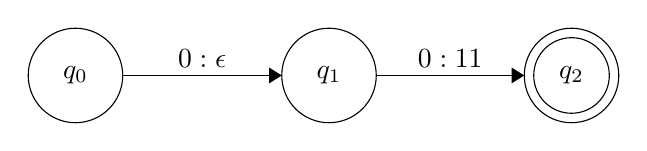
\begin{tikzpicture}[scale=0.2]
	\tikzstyle{every node}+=[inner sep=0pt]
	\draw [black] (13.5,-8) circle (3);
	\draw (13.5,-8) node {$q_0$};
	\draw [black] (29.6,-8) circle (3);
	\draw (29.6,-8) node {$q_1$};
	\draw [black] (45,-8) circle (3);
	\draw (45,-8) node {$q_2$};
	\draw [black] (45,-8) circle (2.4);
	\draw [black] (16.5,-8) -- (26.6,-8);
	\fill [black] (26.6,-8) -- (25.8,-7.5) -- (25.8,-8.5);
	\draw (21.55,-7.5) node [above] {$0:\epsilon$};
	\draw [black] (32.6,-8) -- (42,-8);
	\fill [black] (42,-8) -- (41.2,-7.5) -- (41.2,-8.5);
	\draw (37.3,-7.5) node [above] {$0:11$};
	\end{tikzpicture}
\end{center}

\begin{center}
	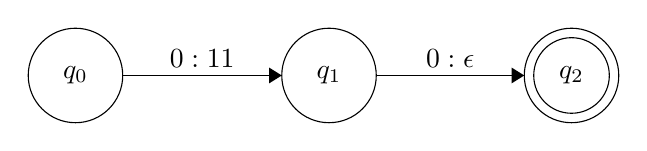
\begin{tikzpicture}[scale=0.2]
	\tikzstyle{every node}+=[inner sep=0pt]
	\draw [black] (13.5,-8) circle (3);
	\draw (13.5,-8) node {$q_0$};
	\draw [black] (29.6,-8) circle (3);
	\draw (29.6,-8) node {$q_1$};
	\draw [black] (45,-8) circle (3);
	\draw (45,-8) node {$q_2$};
	\draw [black] (45,-8) circle (2.4);
	\draw [black] (16.5,-8) -- (26.6,-8);
	\fill [black] (26.6,-8) -- (25.8,-7.5) -- (25.8,-8.5);
	\draw (21.55,-7.5) node [above] {$0:11$};
	\draw [black] (32.6,-8) -- (42,-8);
	\fill [black] (42,-8) -- (41.2,-7.5) -- (41.2,-8.5);
	\draw (37.3,-7.5) node [above] {$0:\epsilon$};
	\end{tikzpicture}
\end{center}

\begin{center}
	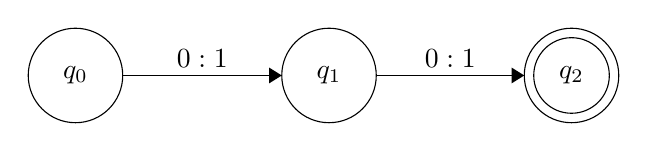
\begin{tikzpicture}[scale=0.2]
	\tikzstyle{every node}+=[inner sep=0pt]
	\draw [black] (13.5,-8) circle (3);
	\draw (13.5,-8) node {$q_0$};
	\draw [black] (29.6,-8) circle (3);
	\draw (29.6,-8) node {$q_1$};
	\draw [black] (45,-8) circle (3);
	\draw (45,-8) node {$q_2$};
	\draw [black] (45,-8) circle (2.4);
	\draw [black] (16.5,-8) -- (26.6,-8);
	\fill [black] (26.6,-8) -- (25.8,-7.5) -- (25.8,-8.5);
	\draw (21.55,-7.5) node [above] {$0:1$};
	\draw [black] (32.6,-8) -- (42,-8);
	\fill [black] (42,-8) -- (41.2,-7.5) -- (41.2,-8.5);
	\draw (37.3,-7.5) node [above] {$0:1$};
	\end{tikzpicture}
\end{center}

All three of those automata are minimal, but only the first one is normalized. The way normalization should work is by pushing all the output as far as possible in the depth of graph. Notice however, that we cannot change this:
\begin{center}
	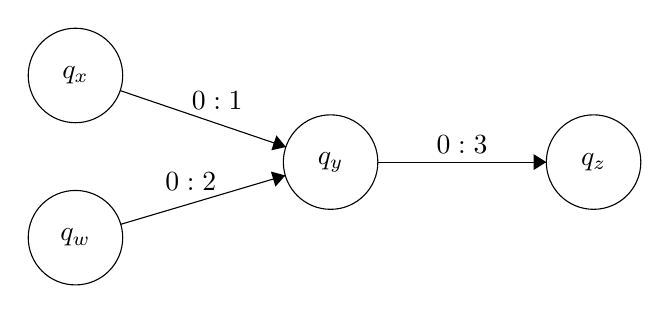
\begin{tikzpicture}[scale=0.2]
	\tikzstyle{every node}+=[inner sep=0pt]
	\draw [black] (13.5,-9.5) circle (3);
	\draw (13.5,-9.5) node {$q_x$};
	\draw [black] (29.7,-15) circle (3);
	\draw (29.7,-15) node {$q_y$};
	\draw [black] (46.4,-15) circle (3);
	\draw (46.4,-15) node {$q_z$};
	\draw [black] (13.5,-19.8) circle (3);
	\draw (13.5,-19.8) node {$q_w$};
	\draw [black] (16.34,-10.46) -- (26.86,-14.04);
	\fill [black] (26.86,-14.04) -- (26.26,-13.3) -- (25.94,-14.25);
	\draw (22.5,-11.72) node [above] {$0:1$};
	\draw [black] (32.7,-15) -- (43.4,-15);
	\fill [black] (43.4,-15) -- (42.6,-14.5) -- (42.6,-15.5);
	\draw (38.05,-14.5) node [above] {$0:3$};
	\draw [black] (16.38,-18.95) -- (26.82,-15.85);
	\fill [black] (26.82,-15.85) -- (25.91,-15.6) -- (26.2,-16.56);
	\draw (20.82,-16.85) node [above] {$0:2$};
	\end{tikzpicture}
\end{center}
into this:
\begin{center}
	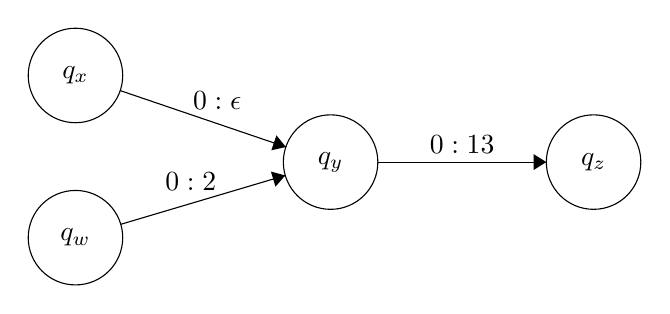
\begin{tikzpicture}[scale=0.2]
	\tikzstyle{every node}+=[inner sep=0pt]
	\draw [black] (13.5,-9.5) circle (3);
	\draw (13.5,-9.5) node {$q_x$};
	\draw [black] (29.7,-15) circle (3);
	\draw (29.7,-15) node {$q_y$};
	\draw [black] (46.4,-15) circle (3);
	\draw (46.4,-15) node {$q_z$};
	\draw [black] (13.5,-19.8) circle (3);
	\draw (13.5,-19.8) node {$q_w$};
	\draw [black] (16.34,-10.46) -- (26.86,-14.04);
	\fill [black] (26.86,-14.04) -- (26.26,-13.3) -- (25.94,-14.25);
	\draw (22.5,-11.72) node [above] {$0:\epsilon$};
	\draw [black] (32.7,-15) -- (43.4,-15);
	\fill [black] (43.4,-15) -- (42.6,-14.5) -- (42.6,-15.5);
	\draw (38.05,-14.5) node [above] {$0:13$};
	\draw [black] (16.38,-18.95) -- (26.82,-15.85);
	\fill [black] (26.82,-15.85) -- (25.91,-15.6) -- (26.2,-16.56);
	\draw (20.82,-16.85) node [above] {$0:2$};
	\end{tikzpicture}
\end{center}
Such operation doesn't preserve disjunctiveity of automaton. Similarly the following two pieces of automata are not equivalent:
\begin{center}
	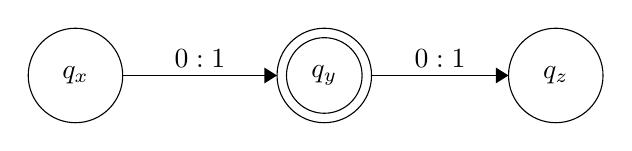
\begin{tikzpicture}[scale=0.2]
	\tikzstyle{every node}+=[inner sep=0pt]
	\draw [black] (13.5,-9.5) circle (3);
	\draw (13.5,-9.5) node {$q_x$};
	\draw [black] (29.3,-9.5) circle (3);
	\draw (29.3,-9.5) node {$q_y$};
	\draw [black] (29.3,-9.5) circle (2.4);
	\draw [black] (44,-9.5) circle (3);
	\draw (44,-9.5) node {$q_z$};
	\draw [black] (16.5,-9.5) -- (26.3,-9.5);
	\fill [black] (26.3,-9.5) -- (25.5,-9) -- (25.5,-10);
	\draw (21.4,-9) node [above] {$0:1$};
	\draw [black] (32.3,-9.5) -- (41,-9.5);
	\fill [black] (41,-9.5) -- (40.2,-9) -- (40.2,-10);
	\draw (36.65,-9) node [above] {$0:1$};
	\end{tikzpicture}
\end{center}
\begin{center}
	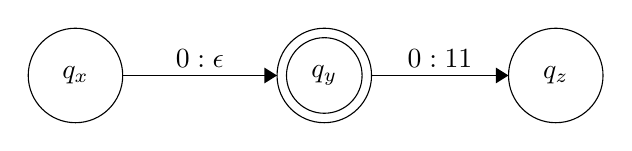
\begin{tikzpicture}[scale=0.2]
	\tikzstyle{every node}+=[inner sep=0pt]
	\draw [black] (13.5,-9.5) circle (3);
	\draw (13.5,-9.5) node {$q_x$};
	\draw [black] (29.3,-9.5) circle (3);
	\draw (29.3,-9.5) node {$q_y$};
	\draw [black] (29.3,-9.5) circle (2.4);
	\draw [black] (44,-9.5) circle (3);
	\draw (44,-9.5) node {$q_z$};
	\draw [black] (16.5,-9.5) -- (26.3,-9.5);
	\fill [black] (26.3,-9.5) -- (25.5,-9) -- (25.5,-10);
	\draw (21.4,-9) node [above] {$0:\epsilon$};
	\draw [black] (32.3,-9.5) -- (41,-9.5);
	\fill [black] (41,-9.5) -- (40.2,-9) -- (40.2,-10);
	\draw (36.65,-9) node [above] {$0:11$};
	\end{tikzpicture}
\end{center}
We can specify it more formally. We seek such automaton that produces all its output as late as possible. Given Mealy automaton $M\in M_\infty$,  we define $\lambda : Q_M \times \Sigma^* \rightarrow \mathbb{ N}$ as:\\
$\lambda_M(q,\epsilon) = 1$ \\ 
$\lambda_M(q,x'x) = (2^{\vert G_M(q,x') \vert+1} - 1)*2^{\lfloor log \lambda_M(\delta_M(q,x'),x) \rfloor }  + \lambda_M(\delta_M(q,x'),x)$ where $x'\in\Sigma$ , $x\in\Sigma^*$ \\
What $\lambda$ does is performing a binary encoding of positions at which automaton printed or read output. For instance given $M(x_0x_1x_2x_3x_4,y_0y_1y_2)$, the output might look like $\lambda(q_0,x_0x_1x_2x_3x_4)=52=00110100_2$ which should be read as:\\
$\underline{0}0110100_2$ - $M$ read $x_0$ (and didn't print anything) \\
$0\underline{0}110100_2$ - next it read $x_1$ and then \\
$00\underline{1}10100_2$ - it printed $y_0$ \\
$001\underline{1}0100_2$ - and $y_1$ (both $y_0$ and $y_1$ were printed on the same edge transitioning over $x_1$)\\
$0011\underline{0}100_2$ - next it read $x_2$\\
$00110\underline{1}00_2$ - and printed $y_2$ \\
$001101\underline{0}0_2$ - then it read $x_3$ \\
$0011010\underline{0}_2$ - and $x_4$ without printing anything more \\
Notice that it actually doesn't matter whether $x_0x_1x_2x_3x_4$ is accepted or rejected. 

Having $\lambda$ we can now define partial order on automata as: \\ 
$M_0 \le_{\lambda} M_1 \iff \forall_{x\in\Sigma^*} \lambda_{M_0}(q_{0M_0},x) \le \lambda_{M_1}(q_{0M_1},x)$ . We will say that an automaton $M\in\mathbb{M}_\infty$ is in normalized form iff there is no smaller (according to $\lambda$) \underline{equivalent} automaton. In other words, we can split $\mathbb{ M}_\infty$ into equivalence classes, introduce on it $\le_\lambda$-order and then all minimal elements within each class are the normalized automata. Obviously there are infinitely many minimal elements (normalized automata) in each class, however there is always  only one automaton that is both minimal (having smallest number of states) and normalized.

It's possible to extend this definition to $\mathbb{ M}_\vee$ by specifying \\ $M_0 \le_{\lambda} M_1  \iff \forall_{t\in T} \pi_t(M_0) \le_{\lambda} \pi_t(M_1)$ where $M_0,M_1\in \mathbb{ M}_\vee$.



\subparagraph{Minimization} For finite state automata the process of minimization is simple thanks to Myhill-Nerode theorem. For non-deterministic FSA minimization becomes PSPACE (and probably NP-hard) problem and on top of that the minimal NFA is not unique. For deterministic single-output Mealy machines there also applies a special version of Myhill-Nerode theorem and minimization procedure is similar to that for deterministic FSA. In case of multi-output deterministic Mealy machines minimization suffers from similar problem to non-deterministic FSA - the minimal automaton is not unique. Any attempt at constructing algorithm that just returns minimal $M_\infty$ is destined to fail if we don't take normalization into account. 

Given automaton $M\in\mathbb{ M}_\infty$ and strings $x,y\in\Sigma^*$, let's define distinguishing extension as pair $(z,w)\in\Sigma^* \times \Gamma^*$ such that exactly one of $(xz,M(x)w)$ or $(yz,M(y)w)$ belongs to $M$. We can then introduce equivalence relation $=_M$ that relates two string only when there doesn't exist any distinguishing extension for them. Formally: \\
$\forall_{x,y\in\Sigma^*} x=_M y \iff \forall_{z:\Sigma^*,w\in\Gamma^*} ((xz,\hat{G}_M(x)w) \in M \iff (yz,\hat{G}_M(y)w) \in M)$ \\
where $\hat{G}_M : \Sigma^* \times Q_M \rightarrow \Gamma^*$ is extended output function (and second argument is by default assumed to be initial state unless explicitly specified otherwise). \\
Notice that $=_M$ will work the same no matter whether $M$ is normalized or not! The only thing that counts is whether $\hat{G}_M(x)w$ and $\hat{G}_M(y)w$ are produced at the moment when $xz$ and $yz$ accept. The output produced by intermediate non-accepting states don't matter because if somewhere at later point there is accepting state, then all normalized and non-normalized (but equivalent) versions should produce the same output. The $\forall$ quantifier is the key!\\
Now, we can use $=_M$ to divide $\Sigma^*$ into equivalence classes. We will show that  iff there are only finitely many such classes then the language is in $\mathbb{ M}_\infty$.  Each class corresponds to one state in minimal version of $M$. Let's say that $[s_0],[s_1],...,[s_{n-1}]$ are the equivalence classes and $[s_i]$ corresponds to state $q_i$ for any $0\le i < n$. Then we can build minimal automaton $N$ using \\
$\delta_N(q_i,s)=q_j \wedge G_N(q_i,s)=s' \iff s_is =_M s_j \wedge \hat{G}_M(s_i)s' = \hat{G}_M(s_is)$ \\
 However, there is one important detail! In order for the $\iff$ equivalence to hold, $M$ must be normalized. Otherwise $ \hat{G}_M$ will introduce ambiguities. If $M$ is not normalized then only one-way implication holds: \\
 $\delta_N(q_i,s)=q_j \wedge G_N(q_i,s)=s' \implies s_is =_M s_j \wedge \hat{G}_M(s_i)s' = \hat{G}_M(s_is)$ \\
 That's because without normalization there might exist two equivalent states of this form:
 \begin{center}
 	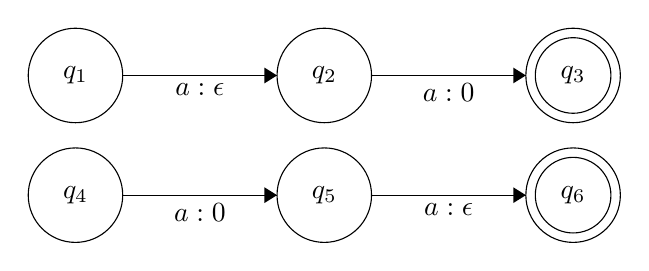
\begin{tikzpicture}[scale=0.2]
 	\tikzstyle{every node}+=[inner sep=0pt]
 	\draw [black] (13.5,-9.5) circle (3);
 	\draw (13.5,-9.5) node {$q_1$};
 	\draw [black] (29.3,-9.5) circle (3);
 	\draw (29.3,-9.5) node {$q_2$};
 	\draw [black] (13.5,-17.1) circle (3);
 	\draw (13.5,-17.1) node {$q_4$};
 	\draw [black] (29.3,-17.1) circle (3);
 	\draw (29.3,-17.1) node {$q_5$};
 	\draw [black] (45.1,-9.5) circle (3);
 	\draw (45.1,-9.5) node {$q_3$};
 	\draw [black] (45.1,-17.1) circle (3);
 	\draw (45.1,-17.1) node {$q_6$};
 	\draw [black] (16.5,-17.1) -- (26.3,-17.1);
 	\fill [black] (26.3,-17.1) -- (25.5,-16.6) -- (25.5,-17.6);
 	\draw (21.4,-17.6) node [below] {$a:0$};
 	\draw [black] (32.3,-17.1) -- (42.1,-17.1);
 	\fill [black] (42.1,-17.1) -- (41.3,-16.6) -- (41.3,-17.6);
 	\draw (37.2,-17.6) node [below] {$a:\epsilon$};
 	\draw [black] (32.3,-9.5) -- (42.1,-9.5);
 	\fill [black] (42.1,-9.5) -- (41.3,-9) -- (41.3,-10);
 	\draw (37.2,-10) node [below] {$a:0$};
 	\draw [black] (16.5,-9.5) -- (26.3,-9.5);
 	\fill [black] (26.3,-9.5) -- (25.5,-9) -- (25.5,-10);
 	\draw [black] (45.1,-9.5) circle (2.4);
 	\draw [black] (45.1,-17.1) circle (2.4);
 	\draw (21.4,-10) node [below] {$a:\epsilon$};
 	\end{tikzpicture}
 \end{center}
Let's say $s_1,s_4 \in \Sigma^*$ are some strings such that $\hat{\delta}_M(s_1) = q_1$ and $\hat{\delta}_M(s_4) = q_4$ . Of course in this example you can clearly see that $s_1 =_M s_4$. So in $N$ we could safely assume $q_1=q_4$. However it's not true that $s_1a =_M s_4$ and neither is $ \hat{G}_M(s_4)0 = \hat{G}_M(s_1a) $.


Also, notice that $s'\in\Gamma^*$ when $M\in\mathbb{ M}_\infty$ but in case of  $M\in\mathbb{ M}_1$ we can narrow it down to $s'\in\Gamma$. \\
This  should conclude the implication that if $=_M$ induced finite number of equivalence classes then $M\in M_\infty$. The opposite implication is trivial. Therefore we obtain a special version of Myhill-Nerode theorem for Mealy machines.\\
The version of this theorem for $\mathbb{ M}_\vee$ is similar but you additionally need to take tapes into account: \\
$\forall_{x,y\in\Sigma^*} x=_M y \iff \forall_{z:\Sigma^*,w\in\Gamma^*} ((xz,\hat{G}_M(x,\hat{F}_M(xz))w) \in M \iff (yz,\hat{G}_M(y,\hat{F}_M(yz))w) \in M)$ \\

\subparagraph{Evaluation of $\mathbb{M}_\rightarrow$} The most basic way of evaluating functional machines is by gradually computing $\gamma$ for all memory cells and all states visited on our way. However, if there are millions of memory cells such process becomes quite inefficient. The alternative method is to split the evaluation into 3 phases:
\begin{enumerate}
	\item for given input string traverse states of automaton, without keeping track of memory cells. This way you first check whether the automaton accepts at all and if it does, then you know which state accepted and which memory cell was used as output.
	\item traverse states backwards, starting from accepting state and ending in initial state. While doing so keep track of sequence of memory cells that leads to the accepting memory cell. This sequence is unambiguous, because given destination cell $t'$, we can precisely know source cell $t$ using $G(q,s,t') = (s',t)$.
	\item traverse automaton forward once again, this time computing output only for the necessary memory cells (there is always only one such cell per each visited state). 
\end{enumerate}
While the original algorithm was $O(xy)$ where $x$ is length of input and $y$ is size of set $T$, this algorithm is only $O(3x) = O(x)$ (if you count memory-cell assignment as basic operation). So it reduces complexity from being quadratic to linear.

\subparagraph{Lossy determinization of $\mathbb{M}$} As we already showed in the proof of $\mathbb{M}_\rightarrow \cap \mathcal{P}(\Sigma^* \times \Gamma^*) =  \mathbb{M} \cap \mathcal{P}(\Sigma^* \rightarrow \Gamma^*)$, there is a lossless way to convert $M \in \mathbb{ M}$ to $N \in \mathbb{M}_\rightarrow$ only when they guarantee deterministic output. However in cases when $M \in \mathbb{ M}$ actually sometimes produces more than one output we need to forcefully choose only one of them. The good news is that we can take advantage of $Q_\psi$. We shall pay extra attention to all those elements $\psi(x) \in Q_\psi$ with more than one accepting state $\vert\psi(x) \cap F_M\vert > 1$. Whenever we encounter it we can just arbitrarily select only one cell $t \in \psi(x)$ to be accepting $F_N(\psi(x)) = t$ and discard the rest. Similarly in cases when multiple $t$ are eligible for $(t',s') \in \check{\delta}_M(t,s)$, we arbitrarily chose one. This should be enough to construct $N$. The rest of procedure remains the same. 

\subparagraph{Detecting non-determinism  of $\mathbb{M}$}
It's easy to detect non-determinism by using the same trick as in lossy determinization of  $\mathbb{M}$. We just search for such $\psi(x)$ where $\vert\psi(x) \cap F_M\vert > 1$. Unfortunately this is not enough, because non-determinism may also arise from ambiguous  $t$ for $(t',s') \in \check{\delta}_M(t,s)$ and it's much more difficult to check. We can in fact show that problem of verifying if non-deterministic automaton always produces at most one output is coNP-complete, by reducing tautology problem to it. 

Given formula $\phi$ in 3-conjunctive normal form over variables $x_1,x_2,...x_n$ we can construct $M \in \mathbb{ M}$ over alphabet $\Sigma=\{0,1\}$, $\Gamma=\{0,1,2\}$ such that $\exists_{x\in\Sigma^*}\vert M(x) \vert >1$ iff $\phi$ is not tautology (alternatively $M$ is functional iff $\phi$ is a tautology).  We will encode assignments using strings $\{0,1\}^n$. For instance for variables $x_1,x_2,x_3$, a string $001$ stands for $x_1=0,x_2=0,x_3=1$. Now suppose $\phi = (X_{h_1}\vee X_{i_1}\vee X_{j_1}) \wedge(X_{h_2}\vee X_{i_2}\vee X_{j_2}) \wedge ... (X_{h_m}\vee X_{i_m}\vee X_{j_m})$, where $X_k$ stands for literal $x_k$ or $\neg x_k$. $\phi$ is not a tautology iff there exists assignment, such that $\phi=0$. 
We can easily build automaton that decides which clauses of $\phi$ are true given some input assignment. In the following structure:


\begin{center}
	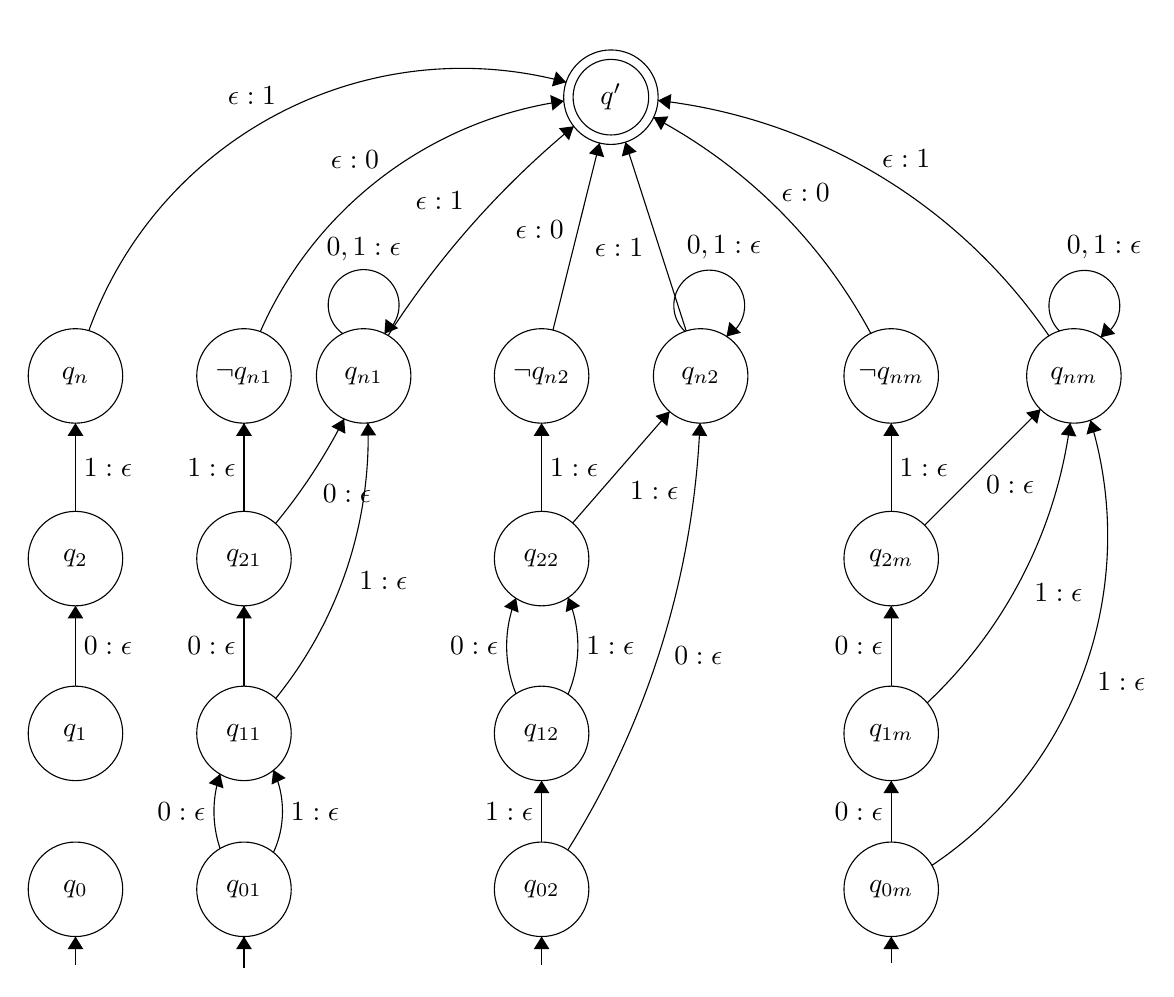
\begin{tikzpicture}[scale=0.2]
	\tikzstyle{every node}+=[inner sep=0pt]
	\draw [black] (14,-55.1) circle (3);
	\draw (14,-55.1) node {$q_{01}$};
	\draw [black] (14,-45.2) circle (3);
	\draw (14,-45.2) node {$q_{11}$};
	\draw [black] (14,-34.1) circle (3);
	\draw (14,-34.1) node {$q_{21}$};
	\draw [black] (32.9,-45.2) circle (3);
	\draw (32.9,-45.2) node {$q_{12}$};
	\draw [black] (14,-22.5) circle (3);
	\draw (14,-22.5) node {$\neg q_{n1}$};
	\draw [black] (32.9,-34.1) circle (3);
	\draw (32.9,-34.1) node {$q_{22}$};
	\draw [black] (32.9,-22.5) circle (3);
	\draw (32.9,-22.5) node {$\neg q_{n2}$};
	\draw [black] (32.9,-55.1) circle (3);
	\draw (32.9,-55.1) node {$q_{02}$};
	\draw [black] (55.1,-55.1) circle (3);
	\draw (55.1,-55.1) node {$q_{0m}$};
	\draw [black] (55.1,-45.2) circle (3);
	\draw (55.1,-45.2) node {$q_{1m}$};
	\draw [black] (55.1,-34.1) circle (3);
	\draw (55.1,-34.1) node {$q_{2m}$};
	\draw [black] (55.1,-22.5) circle (3);
	\draw (55.1,-22.5) node {$\neg q_{nm}$};
	\draw [black] (21.6,-22.5) circle (3);
	\draw (21.6,-22.5) node {$q_{n1}$};
	\draw [black] (43,-22.5) circle (3);
	\draw (43,-22.5) node {$q_{n2}$};
	\draw [black] (66.7,-22.5) circle (3);
	\draw (66.7,-22.5) node {$q_{nm}$};
	\draw [black] (37.3,-4.8) circle (3);
	\draw (37.3,-4.8) node {$q'$};
	\draw [black] (37.3,-4.8) circle (2.4);
	\draw [black] (3.3,-55.1) circle (3);
	\draw (3.3,-55.1) node {$q_0$};
	\draw [black] (3.3,-45.2) circle (3);
	\draw (3.3,-45.2) node {$q_1$};
	\draw [black] (3.3,-34.1) circle (3);
	\draw (3.3,-34.1) node {$q_2$};
	\draw [black] (3.3,-22.5) circle (3);
	\draw (3.3,-22.5) node {$q_n$};
	\draw [black] (12.489,-52.532) arc (-161.17304:-198.82696:7.381);
	\fill [black] (12.49,-47.77) -- (11.76,-48.36) -- (12.7,-48.69);
	\draw (11.59,-50.15) node [left] {$0:\epsilon$};
	\draw [black] (15.862,-47.515) arc (25.01237:-25.01237:6.231);
	\fill [black] (15.86,-47.52) -- (15.75,-48.45) -- (16.65,-48.03);
	\draw (16.95,-50.15) node [right] {$1:\epsilon$};
	\draw [black] (14,-42.2) -- (14,-37.1);
	\fill [black] (14,-37.1) -- (13.5,-37.9) -- (14.5,-37.9);
	\draw (13.5,-39.65) node [left] {$0:\epsilon$};
	\draw [black] (14,-31.1) -- (14,-25.5);
	\fill [black] (14,-25.5) -- (13.5,-26.3) -- (14.5,-26.3);
	\draw (13.5,-28.3) node [left] {$1:\epsilon$};
	\draw [black] (31.279,-42.697) arc (-157.75075:-202.24925:8.046);
	\fill [black] (31.28,-36.6) -- (30.51,-37.15) -- (31.44,-37.53);
	\draw (30.18,-39.65) node [left] {$0:\epsilon$};
	\draw [black] (32.9,-31.1) -- (32.9,-25.5);
	\fill [black] (32.9,-25.5) -- (32.4,-26.3) -- (33.4,-26.3);
	\draw (33.4,-28.3) node [right] {$1:\epsilon$};
	\draw [black] (55.1,-31.1) -- (55.1,-25.5);
	\fill [black] (55.1,-25.5) -- (54.6,-26.3) -- (55.6,-26.3);
	\draw (55.6,-28.3) node [right] {$1:\epsilon$};
	\draw [black] (55.1,-42.2) -- (55.1,-37.1);
	\fill [black] (55.1,-37.1) -- (54.6,-37.9) -- (55.6,-37.9);
	\draw (54.6,-39.65) node [left] {$0:\epsilon$};
	\draw [black] (55.1,-52.1) -- (55.1,-48.2);
	\fill [black] (55.1,-48.2) -- (54.6,-49) -- (55.6,-49);
	\draw (54.6,-50.15) node [left] {$0:\epsilon$};
	\draw [black] (32.9,-52.1) -- (32.9,-48.2);
	\fill [black] (32.9,-48.2) -- (32.4,-49) -- (33.4,-49);
	\draw (32.4,-50.15) node [left] {$1:\epsilon$};
	\draw [black] (34.571,-36.569) arc (23.12817:-23.12817:7.843);
	\fill [black] (34.57,-36.57) -- (34.43,-37.5) -- (35.35,-37.11);
	\draw (35.7,-39.65) node [right] {$1:\epsilon$};
	\draw [black] (14,-60.1) -- (14,-58.1);
	\fill [black] (14,-58.1) -- (13.5,-58.9) -- (14.5,-58.9);
	\draw [black] (32.9,-59.9) -- (32.9,-58.1);
	\fill [black] (32.9,-58.1) -- (32.4,-58.9) -- (33.4,-58.9);
	\draw [black] (55.1,-59.8) -- (55.1,-58.1);
	\fill [black] (55.1,-58.1) -- (54.6,-58.9) -- (55.6,-58.9);
	\draw [black] (21.872,-25.486) arc (1.95545:-38.97672:26.381);
	\fill [black] (21.87,-25.49) -- (21.4,-26.3) -- (22.4,-26.27);
	\draw (21.29,-35.47) node [right] {$1:\epsilon$};
	\draw [black] (20.357,-25.229) arc (-26.88227:-39.58116:35.895);
	\fill [black] (20.36,-25.23) -- (19.55,-25.72) -- (20.44,-26.17);
	\draw (18.98,-29.99) node [right] {$0:\epsilon$};
	\draw [black] (34.87,-31.84) -- (41.03,-24.76);
	\fill [black] (41.03,-24.76) -- (40.13,-25.04) -- (40.88,-25.69);
	\draw (38.49,-29.75) node [right] {$1:\epsilon$};
	\draw [black] (42.958,-25.499) arc (-2.3567:-32.07093:55.329);
	\fill [black] (42.96,-25.5) -- (42.43,-26.28) -- (43.42,-26.32);
	\draw (41.29,-40.23) node [right] {$0:\epsilon$};
	\draw [black] (67.745,-25.31) arc (16.99452:-56.16851:25.176);
	\fill [black] (67.75,-25.31) -- (67.5,-26.22) -- (68.46,-25.93);
	\draw (68.15,-41.88) node [right] {$1:\epsilon$};
	\draw [black] (66.465,-25.489) arc (-7.4019:-46.73337:29.646);
	\fill [black] (66.46,-25.49) -- (65.87,-26.22) -- (66.86,-26.35);
	\draw (64.15,-36.29) node [right] {$1:\epsilon$};
	\draw [black] (57.22,-31.98) -- (64.58,-24.62);
	\fill [black] (64.58,-24.62) -- (63.66,-24.83) -- (64.37,-25.54);
	\draw (62.65,-28.78) node [below] {$0:\epsilon$};
	\draw [black] (20.277,-19.82) arc (234:-54:2.25);
	\draw (21.6,-15.25) node [above] {$0,1:\epsilon$};
	\fill [black] (22.92,-19.82) -- (23.8,-19.47) -- (22.99,-18.88);
	\draw [black] (42.012,-19.68) arc (227.04329:-60.95671:2.25);
	\draw (44.48,-15.08) node [above] {$0,1:\epsilon$};
	\fill [black] (44.64,-20) -- (45.55,-19.76) -- (44.82,-19.07);
	\draw [black] (65.789,-19.654) arc (225.48074:-62.51926:2.25);
	\draw (68.62,-15.09) node [above] {$0,1:\epsilon$};
	\fill [black] (68.4,-20.05) -- (69.32,-19.83) -- (68.61,-19.12);
	\draw [black] (15.038,-19.687) arc (156.29656:98.14817:24.905);
	\fill [black] (34.31,-5.05) -- (33.45,-4.66) -- (33.59,-5.65);
	\draw (21.05,-9.37) node [above] {$\epsilon:0$};
	\draw [black] (23.154,-19.934) arc (147.30412:129.54946:57.538);
	\fill [black] (34.94,-6.65) -- (34,-6.77) -- (34.64,-7.54);
	\draw (27.99,-11.38) node [left] {$\epsilon:1$};
	\draw [black] (33.62,-19.59) -- (36.58,-7.71);
	\fill [black] (36.58,-7.71) -- (35.9,-8.37) -- (36.87,-8.61);
	\draw (34.34,-13.2) node [left] {$\epsilon:0$};
	\draw [black] (42.08,-19.64) -- (38.22,-7.66);
	\fill [black] (38.22,-7.66) -- (37.99,-8.57) -- (38.94,-8.26);
	\draw (39.38,-14.32) node [left] {$\epsilon:1$};
	\draw [black] (40.011,-6.083) arc (62.0949:28.22789:33.387);
	\fill [black] (40.01,-6.08) -- (40.48,-6.9) -- (40.95,-6.02);
	\draw (49.67,-11.44) node [above] {$\epsilon:0$};
	\draw [black] (40.292,-5.008) arc (83.55429:34.34639:34.798);
	\fill [black] (40.29,-5.01) -- (41.03,-5.59) -- (41.14,-4.6);
	\draw (56.05,-9.27) node [above] {$\epsilon:1$};
	\draw [black] (3.3,-42.2) -- (3.3,-37.1);
	\fill [black] (3.3,-37.1) -- (2.8,-37.9) -- (3.8,-37.9);
	\draw (3.8,-39.65) node [right] {$0:\epsilon$};
	\draw [black] (3.3,-31.1) -- (3.3,-25.5);
	\fill [black] (3.3,-25.5) -- (2.8,-26.3) -- (3.8,-26.3);
	\draw (3.8,-28.3) node [right] {$1:\epsilon$};
	\draw [black] (3.3,-59.9) -- (3.3,-58.1);
	\fill [black] (3.3,-58.1) -- (2.8,-58.9) -- (3.8,-58.9);
	\draw [black] (4.149,-19.625) arc (160.13528:74.86663:25.224);
	\fill [black] (34.46,-3.85) -- (33.82,-3.16) -- (33.55,-4.12);
	\draw (14.51,-5.32) node [above] {$\epsilon:1$};
	\end{tikzpicture}
\end{center}


every state $q_{kl}$ stands for "after reading input $x_1x_2x_3...x_k \in \{0,1\}^k$ , partially assigned clause $(X_{h_k}\vee X_{i_k}\vee X_{j_k})$ still has potential to be true". We shall put edge  with label $1:\epsilon$ from state $q_{kl}$ to $q_{(k+1)l}$ iff $\neg x_{k+1}$ is  in the clause. Analogically we put edge $0:\epsilon$ iff $ x_{k+1}$ is  in the clause. The final vertices $q_{n1},..q_{nm}$ tell us which clauses are true for given assignment. Next to them we also designate special vertices $\neg q_{n1},..., \neg q_{nm}$, that collect all the failed false clauses. In the end when automaton reads all $n$ variables, there is an epsilon edge coming from every state $q_{n1},..q_{nm}$ that prints $\epsilon:1$ ( meaning clause is true). Similarly from vertices $\neg q_{n1},..., \neg q_{nm}$ automaton prints $\epsilon:0$ if clause is false. If $\phi$ is a tautology, then for all assignments we will always end up in one of the $q_{n1},..q_{nm}$ and never in $\neg q_{n1},..., \neg q_{nm}$. Therefore the output associated with input sequence $x_1x_2x_3...x_n$ will be unambiguously $1$. If at least one clause fails, then $\phi$ is not tautology and $M$ returns both $0$ and $1$. However there is also a special case, when $\phi$ is contradiction (false for all assignments), we should also get ambiguous output, thanks to states $q_0,...q_n$. $q_n$ is a special state, that can be reached only in one case - when all clauses are simultaneously false. We put edge $1:\epsilon$ transitioning from $q_k$ to $q_{k+1}$ iff $ x_k$ is not present in any clause. Similarly $0:\epsilon$  iff $ \neg x_k$ is not present in any clause. Such construction guarantees us that $\phi$ is tautology iff $M$ is functional. Qed.

 
Notice that if we could find polynomial algorithm for deciding whether non-deterministic automaton is functional, then we would effectively prove that every problem in $coNP=P$ can be decided in polynomial time (so most likely we won't find such algorithm ever). This has profound implications. 
We can is a similar fashion prove that functional union, functional concatenation, functional Kleene closure have no polynomial algorithm. 

Let's prove that given two functional automata $M_0,M_1 \subset \Sigma^* \rightarrow \Gamma^*$, it's impossible to build a polynomial algorithm that computes partial union $M_0 \cup M_1$ such that it yields $M_0 \cup M_1 \subset \Sigma^* \rightarrow \Gamma^*$ iff it's possible, or otherwise returns $\emptyset$ (some special value indicating error). First notice that in the previous proof, every subgraph $q_{0k},q_{1k},q_{2k},...q_{nk},\neg q_{nk}, q'$ corresponding to clause $(X_{h_k}\vee X_{i_k}\vee X_{j_k})$ is guaranteed to be a functional automaton. Similarly the same holds for subgraph $q_0,q_1,q_2,...,q_n,q'$. However if we could easily check if their union is functional, then by applying such union $m$ times (for each clause), then we would effectively check if the whole automaton is functional (which would indicate that $\phi$ is a tautology). Qed.

Analogically for concatenation and Kleene closure WORK IN PROGRESS.

Therefore we can see that having the full power of $\Sigma^* \rightarrow \Gamma^*$ without using lossy determinization comes at the exponential cost (unless $P=NP$).







\subsection{Naive algorithms}
\subparagraph{Weak concatenation in $\mathbb{REG}$}
Given finite state automata $P_0,P_1 \subset \Sigma^*$ the weak concatenation $P_0P_1 $ can be implemented as:
\begin{lstlisting}
$P_m$ := minimize($P_0$)
$P_n$ := minimize($P_1$)
$\square$ := find_sink($P_m$)
$\square$' := find_sink($P_n$)
B := { s $\in \Sigma$ : $\delta_{P_n}$($q_{0P_n}$,s) $\ne$ $\square$' }
if $\square$ = $\emptyset$ $\wedge$ B $\ne$ $\emptyset$
    error
for q $\in$ $F_{P_m}$ 
    for s $\in$ $\Sigma$
        q' := $\delta_{P_m}$(q,s)
        if q' = $\square$ 
            $\delta_{P_m}$(q,s) := $\delta_{P_n}$($q_{0P_n}$,s) 
        else if s $\in$ B
            error
if $q_{0P_n} \in F_{P_n}$            
    $F_{P_m}$ := $F_{P_n} \cup F_{P_m}$
else 
    $F_{P_m}$ := $F_{P_n}$
\end{lstlisting}
$P_m$ and $P_n$ are minimized versions of $P_0$ and $P_1$. We have to minimize them in order to find sink states.  If there is any sink state at all, the it must be unique after performing minimization. The find\_sink procedure tests every state for being the sink (it can be recognized easily because for every character from $\Sigma$ is transitions back to itself). However in case there is no sink the procedure shall return $\emptyset$. If $P_0$ has no such sink then it's obvious that no matter what B is, the weak concatenation will be invalid (unless  $P_1$ has empty base. Empty base occurs only in one scenario - that is when $P_1$ rejects all input and $P_1 = \emptyset$ ). $q_{0P_n}$ is the initial state of $P_n$ and $F_{P_m}$ is the set of final states of $P_m$. For every state from $F_{P_m}$ and character from $\Sigma$ we test if transition leads us to sink state. If that's the case then $\forall_{x\in P_0} \neg \exists_{s\in B} \exists_{t\in\Sigma^*} P_0(xst)$ must hold, because $xs$ leads to sink and for sink there does not exist any $t$ such that $ P_0(xst)$. However, if for a given  character $s$ the final state doesn't transition to sink, it means that there exists some $t$ that accepts (if there was no such $t$ then minimization procedure would merge $\delta_{P_m}(q,s)$ with $\square$). So if there exists such $t$ then we must check if $s$ is in $B$. If the algorithm doesn't fall into error at any point, at the end of execution $P_m$ should hold the structure of $P_0P_1$, because we performed in-place assignment to its transition function $\delta_{P_m}(q,s) := q_{0P_n}$ and effectively merged it with $P_n$.
Also, notice that at the end we must check for one special case - that is when $P_1(\epsilon)=\epsilon$. In such scenario $P_0$ can match too and we should retain its accepting states.
\subparagraph{Weak concatenation in $\mathbb{M}_\infty$} Given $M_0,M_1 \in \mathbb{M}_\vee$, the concatenation $M_0M_1$ can be computed analogically to procedure for $\mathbb{ REG}$. You just need to mutate the output function $G_{P_m}$ at the same time when you mutate $\delta_{P_m}$ . 

\subparagraph{Weak concatenation in $\mathbb{M}_\vee$} This works just the same way as for $\mathbb{M}_\infty$ except you need to handle multiple tapes now. It's more complicated because the tapes of $M_0$ are not the same tapes as those of $M_1$. The naive approach is to first create cartesian product of tapes $T_{M_0} \times T_{M_1}$. Then you change $G_{M_0}$ from $G_{M_0} : Q_{M_0} \times \Sigma \times T_{M_0} \rightarrow \Gamma$, to $G_{M_0} : Q_{M_0} \times \Sigma \times T_{M_0 \times M_1} \rightarrow \Gamma$ where $T_{M_0 \times M_1}$ is isomorphic to $T_{M_0} \times T_{M_1}$. The same must be done for $M_1$ too. Only when both automata use the same tapes you can perform concatenation. However, this approach creates many additional tapes that are in fact redundant. Later we  will show how to remove all of the unnecessary tapes.

\subparagraph{Union in $\mathbb{M}_\vee$}  This works just like union of finite state automata where you additionally zip output tapes of one automaton with output tapes of another. Given automata $M_0,M_1 \subset \Sigma^* \rightarrow \Gamma^*$ union $M_2=M_0 \cup M_1$ can be computed by performing product of states $Q_{M_2} = Q_{M_0} \times Q_{M_1}$. Next you need to zip outputs as $T_{M_2} = T_{M_0} \cup T_{M_1}$  and \\
$\delta_{M_2}((q_{M_0},q_{M_1}),s) = 
(\delta_{M_0}(q_{M_0},s),\delta_{M_1}(q_{M_1},s))$ \\
$G_{M_2}((q_{M_0},q_{M_1}),s,t) = \begin{cases}
G_{M_0}(q_{M_0},s,t)  & \mbox{if }  t \in T_{M_0} \\
G_{M_1}(q_{M_1},s,t)  & \mbox{if }  t \in T_{M_1}
\end{cases}$\\
Last thing to do is to decide accepting states. Remember that deterministic union is defined as $(M_0 \cup M_1)(x,y) \iff M_0(x,y) \vee (\neg \pi_0(M_0)(x) \wedge M_1(x,y))$. Therefore $F_{M_2} : Q_{M_2}  \rightarrow T_{M_2} \cup \{\emptyset\}$ is given by \\
$F_{M_2}((q_{M_0},q_{M_1})) = \begin{cases}
F_{M_0}(q_{M_0})  & \mbox{if }  F_{M_0}(q_{M_0}) \ne \emptyset  \\
F_{M_1}(q_{M_1})  & \mbox{otherwise} 
\end{cases} $ \\
Of course the initial state becomes $q_{0M_2}=(q_{0M_0},q_{0M_1})$.


\subparagraph{Weak Kleene closure in $\mathbb{M}_\vee$} Just like concatenation but we don't need to create Cartesian product of tapes. Given $M \in \mathbb{M}_\vee$, kleene closure can be implemented as

\begin{lstlisting}
$m$ := minimize($M$)
$\square$ := find_sink($m$)
$B$ := { s $\in \Sigma$ : $\delta_m$($q_{0m}$,s) $\ne$ $\square$ }
if $\square= \emptyset\wedge B \ne \emptyset$
    error
for $q\in Q_m$ where $F_m(q) \ne \emptyset$ 
    for $s \in \Sigma$
        $q'$ := $\delta_m$(q,s)
        if $q'$ = $\square$ 
            $\delta_m$(q,s) := $\delta_m$($q_{0m}$,s)
            for $t \in T_m$
                $G_m$(q,s,t) := $G_m$($q_{0m}$,s,t)
        else if s $\in$ B
            error
if $q_{0m} \notin F_m$
   insert new state $q''$ to $Q_m$
   for $s \in \Sigma$
       $\delta_m(q'',s) $ := $\delta_m(q_{0m},s) $
   for $q\in Q_m$
      for $s \in \Sigma$
          if $\delta_m(q,s) = q_{0m} $
              $\delta_m(q,s)$ := $q''$
   insert $q_{0m}$ to $F_m$
\end{lstlisting}
The last part that replaces initial state with $q''$ and adds original initial state to accepting states, is only necessary to express $(\epsilon,\epsilon) \in M^*$. However it's not necessary in case of computing $M^+$. The algorithm for $M^*$ can therefore be largely reused when computing $M^+$, with just the tiny modification that we remove the last 'if' checking for $q_{0m} \notin F_m$ and all the code under that 'if' .
  

\subparagraph{Tape projection $\mathbb{M}_\vee$} This operation is very specific to class $\mathbb{M}_\vee$ but it's required to facilitate other operations. Given automaton $M \in \mathbb{M}_\vee$ with tapes $T_M$, we can take projection $\pi_t$ for any $t\in T_M$ where you can treat $\pi$ as function $T \times (\Sigma^* \rightarrow \Gamma^*) \rightarrow (\Sigma^* \rightarrow \Gamma^*)$. You can compute $M' = \pi_t(M)$ as \\
 $T_{M'} = \{t\}$ \\
 $G_{M'}(q,s,t) = G_M(q,s,t)$ where $t$ is the only possible argument. \\
 $F_{M'}(q) = \begin{cases}
 t & \mbox{if } F_M(q) = t \\
 \emptyset & \mbox{otherwise}
 \end{cases}$ \\
 You can in fact treat $\pi_t$ as $T \times \mathbb{M}_\vee \rightarrow \mathbb{M}_\infty$ in which case you can simplify it to: \\
  $T_{M'}$ is not necessary \\
 $G_{M'}(q,s) = G_M(q,s,t)$ \\
 $q \in F_{M'} \iff F_M(q) = t$ \\

\subparagraph{Composition of $\mathbb{M}_\infty$ with $\mathbb{M}_\vee$} Given automata $M_0 \subset \Gamma^* \rightarrow \Theta^* $ and $M_1 \subset \Sigma^* \rightarrow \Gamma^*$ such that  $M_0 \in \mathbb{M}_\vee$ and $M_1 \in \mathbb{M}_\infty$ the composition $M_2=M_0 \circ M_1 \subset \Sigma^* \rightarrow \Theta^*$ (read it as $M_2(x) = M_0(M_1(x))$ ) can be computed by performing product of states $Q_{M_2} = Q_{M_0} \times Q_{M_1}$. Tapes stay the same as in $T_{M_2} = T_{M_0}$. Then the construction of transition function is as follows:\\
$\delta_{M_2}((q_{M_0},q_{M_1}),s) = 
( \hat{\delta}_{M_0}(q_{M_0},G_{M_1}(q_{M_1},s) ) , \delta_{M_1}(q_{M_1},s) )
$\\
$G_{M_2}((q_{M_0},q_{M_1}),s,t) = \hat{G}_{M_0}(q_{M_0}, G_{M_1}(q_{M_1},s),t )
$\\
Accepting states are given by $F_{M_2}((q_{M_0},q_{M_1})) = F_{M_0}(q_{M_0})$ and initial state is $q_{0M_2} = (q_{0M_0},q_{0M_1})$


\subparagraph{Composition in $\mathbb{M}_\vee$} Given automata $M_0 \subset \Gamma^* \rightarrow \Theta^* $ and $M_1 \subset \Sigma^* \rightarrow \Gamma^*$ composition $M_2=M_0 \circ M_1 \subset \Sigma^* \rightarrow \Theta^*$ (read it as $M_2(x) = M_0(M_1(x))$ ) can be computed by first performing tape projections of $M_0$ for each tape in $T_{M_0}$, then performing composition for them separately and in the end taking union. It can be written as: \\
$M_2 = \bigcup_{t\in T_{M_1}} M_0 \circ \pi_t(M_1)$ \\
Composition is guaranteed to preserve determinism so there is no need to worry about determinism of union operation.


\subparagraph{Normalization in $\mathbb{M}_\infty$} 
The idea behind algorithm is simple. You start with accepting states gradually traverse automaton deeper edge by edge until you hit a vertex that has multiple incoming edges. Then you add  such vertex to queue and repeat algorithm for them. You also need to mark already visited states to prevent algorithm from diverging infinitely. Every time you find a sequence of states $q_1 q_2 q_3 q_4...q_n$ such that every $q_i$ has edge pointing at $q_{i+1}$ and there are no other edges incoming to $q_{i+1}$,  you collect total output accumulated by the sequence of edges between $q_1...q_n$ and replace all of them with epsilons, except for the final edge between $q_{n-1} $ and $q_n$. That last edge should be assigned all the combined output. Once all such sequences are found and all possible outputs are relocated, then you need to go to second phase of algorithm. Now you need to look for nodes that have the same output assigned to all incoming edges. Those are special cases where the output can be further propagated even though there is more than one path to generate such output.
A much less efficient but simpler version of this algorithm is given by:
\begin{lstlisting}
found_change := true
while found_change
   found_change := false
   for $q$ in $Q_M$
      s := longest common suffix of outputs
           on all incoming edges of $q$
      if $s \ne \epsilon$
          remove suffix $s$ from all incoming edges of $q$
          prepend $s$ to output of all outgoing edges
          found_change := true
\end{lstlisting}



\subparagraph{Minimization in $\mathbb{M}_\infty$} 
The main prerequisite for minimization is to normalize first. Then everything becomes easier. Even though theoretically there might exist minimal but not normalized automaton, the algorithm becomes easier when we assume that prior normalization. Then the idea behind algorithm fro minimization becomes simple:

Let's say that $q_1$ and $q_3$ are some arbitrary states in given automaton. 

\begin{center}
	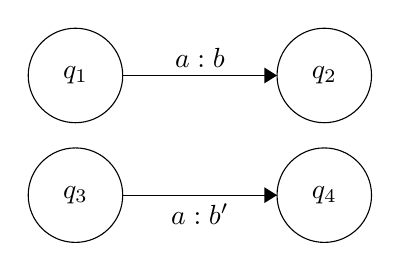
\begin{tikzpicture}[scale=0.2]
	\tikzstyle{every node}+=[inner sep=0pt]
	\draw [black] (13.5,-9.5) circle (3);
	\draw (13.5,-9.5) node {$q_1$};
	\draw [black] (29.3,-9.5) circle (3);
	\draw (29.3,-9.5) node {$q_2$};
	\draw [black] (13.5,-17.1) circle (3);
	\draw (13.5,-17.1) node {$q_3$};
	\draw [black] (29.3,-17.1) circle (3);
	\draw (29.3,-17.1) node {$q_4$};
	\draw [black] (16.5,-9.5) -- (26.3,-9.5);
	\fill [black] (26.3,-9.5) -- (25.5,-9) -- (25.5,-10);
	\draw (21.4,-9) node [above] {$a:b$};
	\draw [black] (16.5,-17.1) -- (26.3,-17.1);
	\fill [black] (26.3,-17.1) -- (25.5,-16.6) -- (25.5,-17.6);
	\draw (21.4,-17.6) node [below] {$a:b'$};
	\end{tikzpicture}
\end{center}

They are equivalent iff they are either equal $q_1=q_3$ or for all inputs $a\in\Sigma$, they produce the same output $b=b'$ and transition  to equivalent states $q_2$ and $q_4$. We can merge all equivalent states that are not equal yet. In order to find equivalent states we can use iterative process. 
Start by finding all states that are equivalent after reading input of length 0. Obviously this yields 2 sets: one containing all accepting states, and the other containing non-accepting states. Then given sets of states that are equivalent after reading input of length $n-1$, we can find states that are equivalent after reading input of lenght $n$, using the condition specified above. We repeat the process until the set of equivalent states becomes constant.
Full algorithm can be written as:
\begin{lstlisting}
M := normalize(M)
equivalent_states := {$F_M$, $Q_M \backslash F_M$}
new_equivalent_states := {} 
while equivalent_states $\ne$ new_equivalent_states
    for equivalent_set in equivalent_states
        for q in equivalent_set
            partition := empty hash map 
            for s in $\Sigma$
                $e$ := $e \in$equivalent_states such that $\delta_M(q,s) \in e$
                if $(e,G_M(q,s))$ not in partition 
                    partition[$(e,G_M(q,s))$] = {}
                insert q to partition[$(e,G_M(q,s))$]
            for $s$ in values of partition
                insert $s$ to new_equivalent_states
     swap new_equivalent_states and equivalent_states 

for eq_class in equivalent_states
    merge all states of $M$ that belong to eq_class
\end{lstlisting}


\subparagraph{Redundant tape elimination in $\mathbb{M}_\vee$} 
WORK IN PROGRESS


\subparagraph{Optimisations}
Very often you don't actually need to compute whole Cartesian products. We will show a couple of ways to speed up some of the algorithms.


Suppose you have two automata $P_0,P_1 \subset \Sigma^*$ and you attempt to evaluate both of them simultaneously and check if they are the same . You start in pair of initial states $(p_{0P_0},p_{0P_1})$ and you look for some signs that would tell you whether $P_0 \ne P_1$. If one of the states is accepting but the other one is not, then that would immediately tell you there is a difference indeed. Another thing to look for is whether one of the states is a sink state, while the other one is not (or in other words, if you still have the potential to accept in the future or not). If so far you couldn't tell any difference then try each transition, one by one. Let's say that you decided to transition over character $s \in \Sigma$ and that lead you to $(p_x,p_y) = (\delta(p_{0P_0},s),\delta(p_{0P_1},s))$. Now you check again whether one of the states is sink or accepts and the other is different. You repeat this search recursively until you either visit all accessible pairs of states $Q_{P_0} \times Q_{P_1}$ or until you hit such pair of states where there is a difference. This is indeed and efficient algorithm for checking equivalence of automata. 

However, we don't have to halt the algorithm after finding first pair of states that differ in functionality.  We can extend this algorithm a little and easily obtain a very efficient procedure for computing union of automata. First, let's change the rules a bit. Now states are distinguishable iff one of them is a sink, and the other is not. We no longer care whether they are accepting. Then let's assign colours to all pairs of states - if they are indistinguishable in functionally then colour them red, otherwise green. Everything is ok, whenever there is a character that transitions you from red pair of states to another red pair. Such transitions mean that so far, we've been evaluating both automata simultaneously and there is still no difference (any of the automata can still potentially accept). However, if there is a transition leading from red to green, then we found a place where only one automaton can still accept, and the other automaton will fall into sink state. Moreover, since it's impossible to escape a sink state, you can notice that every green pair $Q_{P_0} \times Q_{P_1}$ has at least one  element that is a sink state and there is no transition that could lead you from green pair back to red pair. By searching for all reachable pairs of states you effectively computed union of automata, and what's more important, you also marked all indistinguishable states! 


WORK IN PROGRESS


\section{Regular expressions}






\subparagraph{FSA regular expressions}
For FSA, all the standard operations of concatenation, union and Kleene closure form a certain kind of algebra that is often referred to as regular expressions. 
Let $a,b \subset  \Sigma^*$ , then
\begin{itemize}
	\item every $x \in \Sigma$ denotes atomic character. We implicitly treat it as singleton subset of $\Sigma^*$.
	\item $a+b\subset \Sigma^*$ denotes union: $x\in a+b \iff x\in a \vee x\in b$
	\item $ab\subset \Sigma^*$ is concatenation: $x \in ab \iff x=x_0x_1...x_i...x_n \wedge x_0...x_i \in a \wedge x_{i+1}...x_n \in b$
	\item $a^* \subset \Sigma^*$ is Kleene closure: $x\in a^* \iff x=\epsilon \vee x\in a \vee x\in aa \vee x \in aaa \vee ...$
\end{itemize}  

\subparagraph{Mealy regular expressions}
We can easily do the same for non-deterministic Mealy automata. Let $A,B \subset \Sigma^* \times \Gamma^*$, then:
\begin{itemize}
	\item every $x:y \in \Sigma\cup\{\epsilon\} \times \Gamma\cup\{\epsilon\}$ denotes atomic pair. We implicitly treat it as singleton subset of $\Sigma^* \times \Gamma^*$.
	\item $A + B$ is union: $x \in A + B  \iff x \in A \vee x \in B$
\item $AB$ is concatenation: $(x,y)\in AB \iff x=x'x'' \wedge y=y'y'' \wedge (x',y') \in A \wedge (x'',y'') \in B$
\item $A^*$ is Kleene closure: $(x,y)\in A^* \iff (x,y) = (\epsilon,\epsilon) \vee (x,y) \in A \vee (x,y) \in AA \vee ...$
\item given $X\subset \Theta^*\times\Gamma^*$, $Y\subset \Sigma^*\times\Theta^*$  composition $X \circ Y \subset \Sigma^* \times \Gamma^*$ is defined as: $(x,y)\in X \circ Y \iff \exists_{z\in\Theta^*} (x,z)\in Y \wedge (z,y) \in X$
\end{itemize}  
There are also 3 more operations that blend finite state automata and Mealy machines together. Let $a\in\Sigma^*$,$c\subset \Gamma^*$ and $A \in \Sigma^* \times \Gamma^*$, then:
\begin{itemize}
	\item $a:c \subset \Sigma^* \times \Gamma^*$ is product relation $(x,y)\in a:c \iff x\in a\wedge y\in c $
	\item $\pi_0(A)$ is left (input) projection: $x \in \pi_0(A) \iff \exists_{y\in\Gamma^*} (x,y) \in A$
	\item $\pi_1(A)$ is right (output) projection: $y \in \pi_1(A) \iff \exists_{x\in\Sigma^*} (x,y) \in A$
\end{itemize}
However, there is also alternative way to think about those operations. Let $A,B \subset \Sigma^* \times \Gamma^*$, then:
 \begin{itemize}
 	\item $\pi_0(A) \subset \Sigma^* \times \Gamma^*$ is left (input) projection: $\forall_{y\in\Gamma^*} (x,y) \in \pi_0(A) \iff \exists_{y\in\Gamma^*} (x,y) \in A$
 	\item $\pi_1(A) \subset \Sigma^* \times \Gamma^*$ is right (output) projection: $\forall_{x\in\Sigma^*} (x,y) \in \pi_1(A) \iff \exists_{x\in\Sigma^*} (x,y) \in A$
 	\item $A:B \subset \Sigma^* \times \Gamma^*$ is product relation $(x,y)\in A:B \iff (x,y)\in \pi_0(A)\wedge (x,y)\in \pi_1(B)$
 \end{itemize}
Those definitions are equivalent but allow us to operate only on Mealy machines and plain FSA are not necessary. You can easily convert between them. To show this, let's distinguish FSA and Mealy operations by adding subscripts: \\
$+_F$, $\cdot_F$, $^{*F}$,$:_F$,$\pi_{0F}$,$\pi_{1F}$ for union, concatenation and Kleene closure, relation product, left and right projection with FSA operands/outputs.\\ 
$+_M$,$\cdot_M$,$^{*M}$, $\circ$,$:_M$,$\pi_{0M}$,$\pi_{1M}$ for Mealy machines. \\
Then given any formula that uses mix of FSA and Mealy operations, we can define $\phi$ translation that yields formula operating only on Mealy machines:
\begin{itemize}
	\item every atomic character $x\in\Sigma$ becomes atomic pair $\phi(x) = (x,\epsilon)$
	\item every atomic character $y\in\Gamma$ becomes atomic pair $\phi(y) = (\epsilon,y)$
	\item $\phi(a+_Fb) = \phi(a)+_M\phi(b)$ where $a,b\subset \Sigma^*$ or $a,b\subset \Gamma^*$
	\item $\phi(a\cdot_Fb) = \phi(a)\cdot_M\phi(b)$ where $a,b\subset \Sigma^*$ or $a,b\subset \Gamma^*$
	\item $\phi(a^{*F}) = \phi(a)^{*M}$ where $a\subset \Sigma^*$ or $a\subset \Gamma^*$
	\item $\phi(a:_Fb) = \phi(a):_M\phi(b)$ where $a\subset \Sigma^*,b\subset\Gamma^*$
    \item $\phi(\pi_{0F}(a)) = \pi_{0M}(a)$ where $a\subset \Sigma^* \times \Gamma^*$
    \item $\phi(\pi_{1F}(a)) = \pi_{1M}(a)$ where $a\subset \Sigma^* \times \Gamma^*$
    \item $\phi(a\circ b) = a\circ b$ where $a,b\subset \Sigma^* \times \Gamma^*$
\end{itemize} 

It's forth noticing that the following equalities hold:\\
$(ab:c) = (a:\epsilon)(b:c)$ \\
$(a^*:c) = (a^*:\epsilon)(\epsilon:c) = (a:\epsilon)^*(\epsilon:c)$ \\
$(a+b:c) = (a:c)+(b:c)$ \\
where $a,b\in\Sigma^*$ and $c\in\Gamma^*$. Therefore indeed, atomic pairs are enough to build everything else. We do no need atomic characters.


\subparagraph{Kleene algebra}

We can introduce algebra ($\mathcal{A}$,$+$,$\cdot$,$^*$) where $\mathcal{A}$ is some set such that operations of union $+:\mathcal{A}\times\mathcal{A}\rightarrow$, concatenation $\cdot:\mathcal{A}\times\mathcal{A}\rightarrow\mathcal{A}$ and Kleene closure $^*:\mathcal{A} \rightarrow \mathcal{A}$ are closed. Then we admit the following axioms:
\begin{itemize}
	\item Associativity of $+$ \\
	$a + (b + c) = (a + b) + c$ and $a(bc) = (ab)c$
	\item Commutativity of $+$: \\
	$a + b = b + a$
	\item Distributivity \\
	$a(b + c) = (ab) + (ac)$ \\
	$(b + c)a = (ba) + (ca)$
	\item Identity element $0$  \\
	$a + 0 = 0 + a = a$
	\item Identity element $1$  \\
	$a \cdot 1 = 1 \cdot a = a$  
	\item Annihilation: \\
	$a \cdot 0 = 0 \cdot a = 0$
\end{itemize}
Then we can define partial order $a \le b \iff  a+b = b$, which we use to define the rest of axioms:
\begin{itemize}
	\item $1 + a(a^*) \le a^*$ 
	\item $1 + (a^*)a \le a^*$
	\item $ax \le x\implies a^*x \le x$
	\item $xa \le x\implies xa^* \le x$
\end{itemize}
This ends the definition of Kleene algebra. Notice that  $\mathcal{A}$ could be the set of regular languages $\mathcal{A} \subset \mathcal{P}(\Sigma^*)$ with identity elements $\emptyset$ as $0$ and $\epsilon$ as $1$. However, it might also be the set of $\mathbb{ M}$ relations $\mathcal{A} \subset \mathcal{P}(\Sigma^* \times \Gamma^*)$ with $\emptyset$ as $0$ and $(\epsilon:\epsilon)$ as $1$. We shall focus on second case and prove that all the axioms are indeed valid in $\mathbb{ M}$: 
\begin{itemize}
	\item $a + (b + c) = (a + b) + c$ \\
	from definition we know that $(x:y) \in a + (b + c) \iff (x:y) \in a \vee ((x:y) \in b \vee (x:y) \in b) $ but logical disjunction is of course associative by itself.
	\item $ a + b = b + a $ \\
	here similarly, logical disjunction is commutative.
	\item $a(bc) = (ab)c$ \\
	from definition we get $(x:y) \in a(bc) \iff \exists_{x = x_0x_1} \exists_{y = y_0 y_1} (x_0:y_0) \in a \wedge (x_1:y_1) \in bc \iff \exists_{x = x_0x_1x_2} \exists_{y = y_0 y_1y_2} (x_0:y_0) \in a \wedge ((x_1:y_1) \in b \wedge (x_2:y_2) \in c)$ but logical conjunction is of course associative. 
	\item $a(b + c) = (ab) + (ac)$ \\
	from definition we get $(x:y) \in a(b+c) \iff \exists_{x = x_0x_1} \exists_{y = y_0 y_1} (x_0:y_0) \in a \wedge (x_1:y_1) \in b+c \iff \exists_{x = x_0x_1} \exists_{y = y_0 y_1} (x_0:y_0) \in a \wedge ((x_1:y_1) \in b \vee (x_1:y_1) \in c)$, but logical disjunction and conjunction are distributive with respect to each other. 
	\item $(b + c)a = (ba) + (ca)$ \\
	this can be derived analogically to earlier proofs.
	\item $a + \emptyset = \emptyset + a = a$ \\
	from definition we get $(x:y) \in a + \emptyset \iff (x:y) \in a \vee (x:y) \in \emptyset$, but obviously $(x:y) \in \emptyset$ is false therefore $(x:y) \in a + \emptyset \iff (x:y) \in a$. 
	\item $a (\epsilon:\epsilon) = (\epsilon:\epsilon) a = a$  \\
	from definition we get $(x:y) \in a (\epsilon:\epsilon) \iff  \exists_{x = x_0x_1x_2} \exists_{y = y_0 y_1y_2} (x_0:y_0) \in a \wedge (x_1:y_1) = (\epsilon:\epsilon)$, but since $(x_1:y_1) = (\epsilon:\epsilon)$, then $x=x_1$ and $y=y_1$ so that leaves us with  $(x:y) \in a (\epsilon:\epsilon) \iff   (x:y) \in a $
	\item $a\emptyset = \emptyset a = \emptyset$ \\
	from definition we get $(x:y) \in a \emptyset \iff  \exists_{x = x_0x_1x_2} \exists_{y = y_0 y_1y_2} (x_0:y_0) \in a \wedge (x_1:y_1) \in \emptyset$, but since $(x_1:y_1) \in \emptyset$ is always false, that leaves us with the entire right side of equivalence always false. Therefore the equivalence will be true only when $(x:y) \in a \emptyset$ is always false. That means, nothing belongs to $a \emptyset$, so $a \emptyset = \emptyset$.
\end{itemize}

One of the most important properties of such algebra is Arden's theorem. It says that:
if $x = ax+b$ then $x=a^*b$\\
The proof is quite simple (although not very formal): \\
if $x = ax+b$ then of course $x = a(ax+b)+b = aax+ab+b$. We can keep substituting $x$ infinitely to obtain series $x = b + ab + a^2b + a^3b + ... = (1 + a + a^2 + a^3 + ...)b$ and you should notice that $(1 + a + a^2 + a^3 + ...)$ is the exact definition of $a^*$. Therefore $x=a^*b$.


You can prove analogical property for $x = xa+b \implies x=ba^*$ and even for $x = cxa+b \implies x=c^nba^n$, but it's not really important for our purposes. The reason why Arden's theorem is so important is because it allows us to convert every Mealy machine to some regular expression. Here is how it can be done:

Assume that we are given some automaton $M\in \mathbb{ M}$ with $\delta : Q \times (\Sigma \cup \{\epsilon \}) \rightarrow Q \times \Gamma^*$. We can associate certain relation with each of its states. $q \in Q$ is "equivalent" to relation $l_q \subset \Sigma^* \times \Gamma^*$ such that every pair $(x,y) \in \Sigma^* \times \Gamma^*$ belongs to $(x,y) \in l_q$ iff it would be accepted by automaton $M$ with $q$ as initial state. Every transition $  \delta(q,s) = (q',s')$ can be then associated with regular expressions $q(s:s') < q'$. We can present it visually as:



\begin{center}
	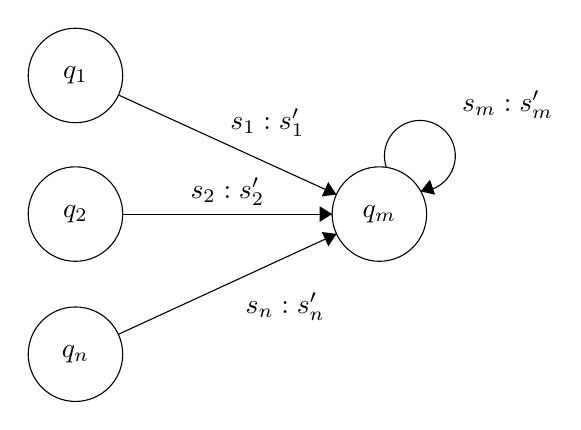
\begin{tikzpicture}[scale=0.2]
	\tikzstyle{every node}+=[inner sep=0pt]
	\draw [black] (46.7,-16.1) circle (3);
	\draw (46.7,-16.1) node {$q_m$};
	\draw [black] (27.4,-7.3) circle (3);
	\draw (27.4,-7.3) node {$q_1$};
	\draw [black] (27.4,-16.1) circle (3);
	\draw (27.4,-16.1) node {$q_2$};
	\draw [black] (27.4,-25) circle (3);
	\draw (27.4,-25) node {$q_n$};
	\draw [black] (30.13,-8.54) -- (43.97,-14.86);
	\fill [black] (43.97,-14.86) -- (43.45,-14.07) -- (43.04,-14.98);
	\draw (39.58,-11.18) node [above] {$s_1:s_1'$};
	\draw [black] (30.4,-16.1) -- (43.7,-16.1);
	\fill [black] (43.7,-16.1) -- (42.9,-15.6) -- (42.9,-16.6);
	\draw (37.05,-15.6) node [above] {$s_2:s_2'$};
	\draw [black] (30.12,-23.74) -- (43.98,-17.36);
	\fill [black] (43.98,-17.36) -- (43.04,-17.24) -- (43.46,-18.15);
	\draw (40.72,-21.08) node [below] {$s_n:s_n'$};
	\draw [black] (47.145,-13.145) arc (199.16362:-88.83638:2.25);
	\draw (54.85,-10.06) node [above] {$s_m:s_m'$};
	\fill [black] (49.32,-14.66) -- (50.24,-14.87) -- (49.91,-13.92);
	\end{tikzpicture}
\end{center}
$ l_{q_1}(s_1:s_1') \le l_{q_m}$, \\
$ l_{q_2}(s_2:s_2') \le l_{q_m}$, \\
 ...,  \\
$ l_{q_n}(s_n:s_n') \le l_{q_m}$,\\
$l_{q_m}(s_m:s_m') \le l_{q_m}$. \\
Indeed it holds that: \\
$l_{q_m} =  l_{q_1}(s_1:s_1') + l_{q_2}(s_2:s_2') + .. + l_{q_n}(s_1:s_n') + l_{q_m}(s_m:s_m')$ \\
and you can build such equations for every state. This should yield entire system of linear equations that can be solved using method similar to Gaussian elimination in some sense. You could represent this system in such a way: \\
$l_{q_0} = l_{q_0}p_{00} + l_{q_1}p_{10} + l_{q_2}p_{20} + ...$ \\
$l_{q_1} = l_{q_0}p_{01} + l_{q_1}p_{11} + l_{q_2}p_{21} + ...$ \\
$l_{q_2} = l_{q_0}p_{02} + l_{q_1}p_{12} + l_{q_2}p_{22} + ...$ \\
$...$ \\
where each $p_{ij}$ corresponds to some pair of the form $p_{ij} \subset (\Sigma \cup \{\epsilon \}) \times \Gamma^*$ such that $\delta(q_j,\pi_0(p))=(q_i,\pi_1(p))$, or otherwise in cases when there is no transition from $q_j$ to $q_i$ then $p=\emptyset$. Notice that we can apply Arden's theorem to convert \\
$l_{q_0} = l_{q_0}p_{00} + l_{q_1}p_{10} + l_{q_2}p_{20} + ...$ \\
into \\
$l_{q_0} =  (l_{q_1}p_{10} + l_{q_2}p_{20} + ...)p_{00}^*$ \\
which can also be written as: \\
$l_{q_0} =  l_{q_1}p_{10}p_{00}^* + l_{q_2}p_{20}p_{00}^* + ...$ \\
Next you can substitute $ l_{q_0}$ in all other equations, yielding: \\
$l_{q_1} = l_{q_1}(p_{11} + p_{10}p_{00}^*p_{01} )+ l_{q_2}(p_{21} + p_{20}p_{00}^*p_{01})+... $ \\
$l_{q_2} = l_{q_1}(p_{12} + p_{10}p_{00}^*p_{02}) + l_{q_2}(p_{22} + p_{20}p_{00}^*p_{02})+ ...$ \\
$...$\\
This way we effectively got rid of one column and row. By repeating this procedure iteratively we will eventually reach just one single equation. However, notice that it's not the end. Currently we arranged all equations in order starting from $q_0$ going up to the last state, because such arrangement looks simpler and more tidy. Unfortunately as a result we will obtain equation describing the last state, not the initial state $q_0$. We can fix it be making a simple rearrangement of equations. We just need to make sure that we never substitute $q_0$.






\subparagraph{Non-empty initial tape}
We already discussed $\#$ as end-of-string marker and showed that it increases expressive power of deterministic automata. However, there exists alternative approach to expressing $\epsilon$ mappings (and it's better suited for use in regular expressions). The trick is to start execution of automaton, with the output tape initialized with some specific symbols.

In case of $M \in \mathbb{ M}_\infty$ this is equivalent to appending $\epsilon : y$ if front of $M$. For instance let's say \\
$M = (a:b)^* = \{ (\epsilon,\epsilon), (a,b), (aa,bb),... \}$, \\
then after prepending $(\epsilon : b)$ you would get \\
$(\epsilon : b)M =  (\epsilon : b)(a:b)^* = \{(\epsilon,b), (a,bb), (aa,bbb),...  \}$. \\
Weak concatenation still works fine with it, however, the real problem becomes Kleene closure. If $(\epsilon:y) \in M$ then $(\epsilon^0:y^0) ,(\epsilon^1:y^1), (\epsilon^2:y^2) , ... \in M$ but because $y\ne \epsilon$ it soon turns out that $\epsilon^2 = \epsilon$ and $y^2 \ne y$, which leads to infinitely many outputs associated with $\epsilon$. Similarly, union becomes severely limited. Any two automata with different $\epsilon$ mappings are immediately incompatible for union operation (so you are forced to resort to $\oplus$ operation). However, it's actually not as bad as it seems. Weak Kleene closure, weak concatenation and partial union still work in all those cases that do not use $\epsilon$ mappings. Allowing for tape preallocation doesn't break existing properties of $\mathbb{ M}_\infty$. It in fact increases expressive power.  Therefore let's quickly revise all previous operations/algorithms and see how they become affected. 

First of all, notice that many automata with preallocated tape can in fact be easily turned into equivalent ones with empty initial tape. You just need to check if the initial state  $q_0$ is accepting. If it's not, you can take the preallocated tape output and put it on all outgoing edges of initial state. This way you will start with empty tape. (The only complication is when $q_0 $ also has some incoming transitions. In such case, you need to duplicate initial state, before appending output to it's transitions.) If initial state is at the same time accepting, you cannot remove preallocated output and you need to leave the automaton as is. 
\begin{itemize}
	\item Normalization can be performed the same way as previously, but you should first attempt to reduce initial tape to empty if possible.
	\item Union (both partial $\cup$ and non-commutative $\oplus$) will work the same as previously except you need to make sure that both automata have the same initial tape contents. If they are different (and their reduction is not possible) then union is undefined. Notice that even in case of $\oplus$ union, it's not possible to just prioritize tape of left argument over the right one. Therefore $\oplus$ must become partial as well. 
	\item 
	Weak concatenation $M_0 M_1 = M_2$ should work similarly with some tiny modifications. Initial tape contents of $M_2$ should be the same as contents of $M_0$. For each accepting state of $M_0$, we need to redirect transitions. All those transition that goes over character belonging to base of $M_1$,  need to be redirected to initial state of $M_1$. However, this time we additionally append to output of those transitions, the initial tape contents of  $M_1$.
	\item Weak Kleene closure cannot work if $\epsilon$ mapping is accepted and is a non-empty string. Therefore we either can reduce the automaton to equivalent one with empty initial tape, or we cannot perform Kleene closure.
	
\end{itemize}


This should cover most essential properties of $\mathbb{ M}_\infty$. Now we should consider $\mathbb{ M}_\vee$.  In this case we can no longer just append $(\epsilon:y)$ in front. Instead we need to define \\
$G(q_0,\epsilon) : T \rightarrow \Gamma^*$ \\
to be the initial contents of each tape. Many such  automata can be reduced to equivalent automata with empty initial tapes, in the same way as we did it for $\mathbb{ M}_\vee$, except this time if $q_0$ is accepting state, then we check which tape accepts. We need to leave that one tape with preallocated contents, however all other tapes can be made empty and their contents would be appended to respective outputs of $q_0$ transitions. (And if $q_0$ has incoming transitions, then you need to duplicate $q_0$ before modifying its outputs). Therefore we can conclude that we don't even need $G(q_0,\epsilon)$. It's enough to just have initial pair $T \times \Gamma^*$, because preallocating only one tape suffices. We will use $(t_\epsilon,s_\epsilon) \in T \times \Gamma^*$ to denote the one designated  tape and it's initial contents (all other tapes are empty). 
\begin{itemize}
	\item Normalization can be performed the same way are previously, but you should first attempt to reduce initial tapes to empty if possible.
	\item Union (both partial $\cup$ and non-commutative $\oplus$) will work the same as previously except you need to make sure that both automata have the same initial contents in their respective initial tapes $t_\epsilon$. If they are different then union is undefined. Notice that in case of $\oplus$ union, we could prioritize $t_\epsilon$ of left argument over the right one. Therefore $\oplus$ is not partial.
	\item Weak concatenation $M_0 M_1 = M_2$ should work similarly with some tiny modifications. You need to perform Cartesian product of tapes. Then initial tape contents of $M_2$ should be the same as respective contents of $M_0$. For each accepting state of $M_0$, we need to redirect transitions. All those transition that go over character belonging to base of $M_1$,  need to be redirected to initial state of $M_1$. However, this time we additionally append to output of those transitions, the initial tape contents of  $M_1$ (most tapes are initially empty except for $t_{\epsilon M_1}$). You should also take extra caution in case when both $M_0$ and $M_1$ have some mapping for  $\epsilon$, because then the mapping for $M_2$ is concatenation of both. And when you perform Cartesian  product of tapes, some of them will need to be preallocated with $s_{\epsilon M_0}$, while there will be one tape preallocated with concatenation $s_{\epsilon M_0}s_{\epsilon M_1}$ of both.
	\item Weak Kleene closure cannot work if $\epsilon$ mapping is accepted and is a non-empty string. Therefore we either can reduce the automaton to equivalent one with all initial tapes empty, or we cannot perform Kleene closure at all. 
	
	This should conclude the procedure for converting Mealy machines to regular expressions. At the same time it's also a constructive proof that power of regular expressions is at least as expressive as that of $\mathbb{ M}$ (in fact their power is equal).
	
\end{itemize}

\subparagraph{Weak union} We can further weaken partial union by using the same mechanism as in weak concatenation and weak Kleene closure. Weak union $M_0 \cup' M_1$ is defined iff base of $M_0$ and base of $M_1$ have no common elements. It may seam like weak union is more limited in expressive power than partial union but it's not entirely true.

\subparagraph{Regular expressions for $\mathbb{ M}_\infty$} We already showed how Kleene algebra can work for $\mathbb{ M}$ (and it works almost the same for FSA). Now we will investigate deterministic $\mathbb{ M}_\infty$ automata. Since we already know that $\mathbb{ M}_\infty \subsetneq \mathbb{ M}$ and regular expressions are equivalent in power to $\mathbb{ M}$, we could intuitively conclude that regular expressions for $\mathbb{ M}_\infty$ should be different (and less powerful). Our best option is to use weak union, weak concatenation and weak Kleene closure. Unfortunately it has one serious drawback. The syntactic correctness of formulas does no longer correspond to semantic correctness. For instance the formula $(a:\epsilon)^*$ is correct both syntactically and semantically, but formula $((a:\epsilon)^*)^*$ is only valid in syntactic sense. Because of the partial nature of the three fundamental operations, many cases become invalid semantically. The most obvious way to validate formula is of course by attempting to build corresponding automaton. However, this might be an expensive operation. We could propose a more efficient way that validates formula without evaluating it.

The idea is quite simple. Start with atomic pairs/characters and gradually traverse syntax tree while keeping track of base, co-base and initial $t_\epsilon$ tape of each subformula  (in case of $\mathbb{ M}_\infty$, $t_\epsilon $ is just the single output tape that's available). Let's denote base alphabet of formula $a$ as $\alpha(a)$ and co-base alphabet as $\omega(a)$ and $\epsilon$ mapping that $a$ accepts as $\mathcal{T}(a)$. Then:
\begin{itemize}
	\item For any atomic $x:y\in (\Sigma \cup \{\epsilon\} )\times(\Gamma\cup\{\epsilon\})$ we get 
	\begin{itemize}
		\item $\alpha(x:y) = \begin{cases}
		\{x\} & x\ne\epsilon \\
		\emptyset & x=\epsilon
		\end{cases}$ 
		\item $ \omega(x:y) = \emptyset$
		\item $\mathcal{T}(x:y) = \begin{cases}
		y & x=\epsilon \\
		\emptyset & x\ne \epsilon
		\end{cases}$
	\end{itemize} 
	\item For subformula $a+b$ we get 
	\begin{itemize}
		\item $\alpha(a+b) = \alpha(a) \cup \alpha(b) $
		\item $\omega(a+b) = \omega(a) \cup \omega(b) $
		\item $\mathcal{T}(a) \cup \mathcal{T}(b) = \mathcal{T}(a+b) $ 
	\end{itemize} 
   And we require that $\vert \mathcal{T}(a) \cup \mathcal{T}(b)  \vert \le 1$ and $\alpha(a) \cap \alpha(b) = \emptyset$ or otherwise the union is undefined.
	\item For subformula $ab$ we get
	\begin{itemize}
		\item $\alpha(ab) = \begin{cases}
		\alpha(a) & \mathcal{T}(a)=\emptyset \\
		\alpha(a) \cup \alpha(b) & \mathcal{T}(a)\ne\emptyset
		\end{cases} $ \\
		because if $(\epsilon:y) \notin a$ then every string in $ab$ can start only with the same characters as any string in $a$. However, if $a$ accepts $\epsilon$, then we might go straight to matching $b$ and this way there might exist string in $ab$ that starts with letter that is not in base of $a$, but instead is in base of $b$.
		\item $\omega(ab) = \begin{cases}
		\omega(b)  & \mathcal{T}(b)=\emptyset \\
		\omega(a) \cup \omega(b)  & \mathcal{T}(b) \ne \emptyset \\
		\end{cases}$ \\
		because if $\epsilon$ is not accepted by $b$, then every string matched by $ab$ must have non-empty suffix accepted by $b$. Then every longer superstring can only take further transitions within $a$ and there are no transitions that go from $b$ back to checking $a$. Therefore co-base of $b$ becomes co-base of $ab$. However, in cases when $\epsilon$ is accepted by $b$, all accepting states of $a$ must also be accepting states of $ab$, and there might be transitions that take you further to other states within $a$. 
		\item $\mathcal{T}(ab) = \begin{cases}
		\mathcal{T}(a)  & \mathcal{T}(b)=\emptyset \\
		\mathcal{T}(a)\mathcal{T}(b)  & \mathcal{T}(b) \ne \emptyset \\
		\end{cases} $ 
	\end{itemize} 
    We also require $\alpha(b)\cap\omega(a)=\emptyset$ for weak concatenation to work. 
	\item For subformula $a^*$ we get 
	\begin{itemize}
		\item $\alpha(a^*) = \alpha(a)$
		\item $\omega(a^*) =   \alpha(a) \cup \omega(a) $
		\item $\mathcal{T}(a^*) = \emptyset$ and we require $\mathcal{T}(a) = \emptyset$
	\end{itemize} 
    We also require $\alpha(a)\cap\omega(a)=\emptyset$ for weak Kleene closure to work.
\end{itemize}
This allows us to quickly check if all weak Kleene closures, weak concatenations and weak unions are valid. Notice that if we used partial union, then validation would become much more complicated.



\subparagraph{$\mathbb{ M}_\vee$ to $\mathbb{ M}_\infty$ reduction}
We can reduce every disjunctive automaton to certain multi-output automaton, that is not equivalent, but whose output language is homomorphic. We use interleaved pairs to encode multiple tapes into a single one. The exact construction is simple:

Given $M \in \mathbb{ M}_\vee$ with set of tapes $T$ we can produce automaton $N \in \mathbb{ M}_\infty$ with homomorphism $\phi$ that turns state of all the $M$'s output tapes to some string produced by $N$, which can be described as  $\phi : (\Gamma_M^*)^{\vert T \vert} \rightarrow \Gamma_N^*$. First we need to duplicate the output alphabet $\Gamma_M$ for each tape $t\in T$. We shall use $\Gamma^t_M$ to denote alphabet $\Gamma_M$ for corresponding tape $t$, and for every $s \in \Gamma_M$ and $t\in T$ there is $s^t \in \Gamma^t_M$. Then the output alphabet of $N$ is given by $\Gamma_N = \bigcup_{t\in T}\Gamma_M^t$. The homomorphism converts strings of $\Gamma_N$ to tuples $\Gamma_M^{t_0} \times \Gamma_M^{t_1} \times ... \times  \Gamma_M^{t_n} $ therefore it can be seen as a certain interleaved encoding $\phi : (\Gamma_M^{t_0} \times \Gamma_M^{t_1} \times ... \times  \Gamma_M^{t_n}) \rightarrow \mathbb{ S}(\Gamma_M^{t_0} \times \Gamma_M^{t_1} \times ... \times  \Gamma_M^{t_n})$ and the automata themselves represents relations of the form $N \subset  \Sigma^* \rightarrow \mathbb{S}(\Gamma_M^{t_0} \times \Gamma_M^{t_1} \times ... \times  \Gamma_M^{t_n})$ and $M \subset \Sigma^* \rightarrow (\Gamma_M^{t_0} \times \Gamma_M^{t_1} \times ... \times  \Gamma_M^{t_n})$ where $\forall_{s\in\Sigma^*} \phi(M(s))=N(s)$. Then the output function of $N$ becomes $G_N(q,s) = G(q,s,t_0) \cdot G(q,s,t_1) \cdot ... \cdot G(q,s,t_n)$. States can stay the same as $Q_N = Q_M$, $q_{0N} = q_{0M}$. Moreover $N$ should accept whenever any of the $M$'s tapes accept $F_N = \{ q \in Q_ N: F_M(q) \ne \emptyset \}$.  

Such approach will be of great importance when investigating properties of regular expressions for $\mathbb{ M}_\vee$, because we can operate on strings produced by $N$ just as if we operated all tapes of $M$ simultaneously.

\subparagraph{ Weak Kleene algebra}  In case of $\mathbb{ M}_\infty$, regular expressions are limited by weak concatenation, weak Kleene closure and weak union. We can use those operations to build system similar to Kleene algebra with the only exception that, almost every axiom needs to take partiality of operations into account. For instance the axiom of commutativity would now look like this: \\
$a + b = b + a \iff \alpha(a) \cap \alpha(b) = \emptyset$

Because of this, Arden's theorem becomes: \\
$(x=ax+b \implies x = a^*b) \iff \alpha(a) \cap \omega(a) \cap \alpha(b) = \emptyset$
We can prove it as: 

\subparagraph{Glushkov's construction for Mealy machines}

We already know how to build regular expressions for $\mathbb{M}_\vee$ machines and how to convert one. We also showed algorithms for performing all the basic operations of union, concatenation and Kleene closure. While it's easy to notice that  those algorithms are polynomial (which is great by itself!), the bad news is that many of them perform Cartesian products of states or tapes. Therefore if given two automata with respective number of states/tapes $n$ and $m$, then performing those operations can be done in $O(mn)$ time. Now it gets more complicated when we compute entire regular expressions. let's say that we perform union $k$ times for automata $M_1 \cup M_2 \cup ... \cup M_k \subset \Sigma^* \rightarrow \Gamma^*$. Then Cartesian product of $Q_1 \times Q_2 \times... Q_k$ yields exponential number of states with respect to $k$. Good news is that we can make huge optimisations with help of Glushkov's construction.



\section{Further extensions WORK IN PROGRESS}

\paragraph{Multitape} automata can be expressed in a variety of creative ways. The most obvious way is to use more complicated version of $\delta$ that looks more or less like this: $Q \rightarrow [ (\Sigma_1 ,  \Sigma_2 ,  \Sigma_3 , ... , Q , [ \Gamma ])]$. However, it greatly complicates all algorithms. On top of that, even though we might have total order on each alphabet $\Sigma_i$ by itself, there is no good total order for tuples $(\Sigma_1 ,  \Sigma_2 ,  \Sigma_3 , ... )$ . We could use lexicographic ordering but it actually makes matters worse. (Previously we could express ranges $s ... s'$ for $s\le s':\Sigma$ as list of form $[ ...,(s-1,\square),(s',q), ...]$, but now there is no way to express ranges $s_1...s_1' \times s_2...s_2'$ with constant asymptotic complexity of memory). It is possible cantor's pairing function to compress tuples $(\Sigma_1 ,  \Sigma_2 ,  \Sigma_3 , ...) $ into a new alphabet $\Sigma$ but it only delays problems instead of solving them. A far better approach is to forget about reading all tapes simultaneously, and instead combine all tapes into a single tape by interleaving all of them. Automaton that alternates between two tapes (and possibly two different alphabets) must keep track of currently used tape. For this reason there need to be  states of different kinds. We will illustrate it with example: \\
\\
Let's say there are two tapes, first with alphabet $\Sigma_0=\{ a , b\}$ and second with  $\Sigma_1=\{A,B\}$ . States that read from first tape will be marked red. Those that read from second are blue.

\begin{center}
	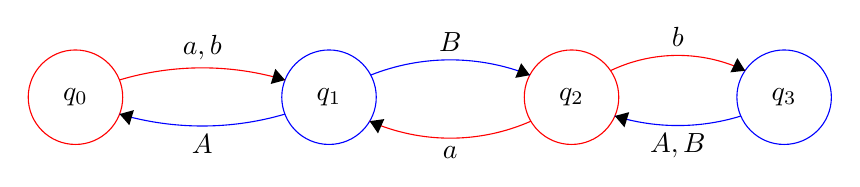
\begin{tikzpicture}[scale=0.2]
	\tikzstyle{every node}+=[inner sep=0pt]
	\draw [red] (13.5,-8) circle (3);
	\draw (13.5,-8) node {$q_0$};
	\draw [blue] (29.6,-8) circle (3);
	\draw (29.6,-8) node {$q_1$};
	\draw [red] (45,-8) circle (3);
	\draw (45,-8) node {$q_2$};
	\draw [blue] (58.5,-8) circle (3);
	\draw (58.5,-8) node {$q_3$};
	\draw [red] (16.29,-6.907) arc (106.6952:73.3048:18.309);
	\fill [black] (26.81,-6.91) -- (26.19,-6.2) -- (25.9,-7.16);
	\draw (21.55,-5.64) node [above] {$a,b$};
	\draw [blue] (32.245,-6.596) arc (111.67997:68.32003:13.685);
	\fill [black] (42.36,-6.6) -- (41.8,-5.84) -- (41.43,-6.77);
	\draw (37.3,-5.13) node [above] {$B$};
	\draw [blue] (26.802,-9.073) arc (-73.63011:-106.36989:18.635);
	\fill [black] (16.3,-9.07) -- (16.92,-9.78) -- (17.21,-8.82);
	\draw (21.55,-10.33) node [below] {$A$};
	\draw [red] (42.423,-9.522) arc (-66.20209:-113.79791:12.696);
	\fill [black] (32.18,-9.52) -- (32.71,-10.3) -- (33.11,-9.39);
	\draw (37.3,-11.1) node [below] {$a$};
	\draw [red] (47.469,-6.317) arc (115.60241:64.39759:9.906);
	\fill [black] (56.03,-6.32) -- (55.53,-5.52) -- (55.09,-6.42);
	\draw (51.75,-4.84) node [above] {$b$};
	\draw [blue] (55.755,-9.195) arc (-72.81583:-107.18417:13.556);
	\fill [black] (47.75,-9.19) -- (48.36,-9.91) -- (48.66,-8.95);
	\draw (51.75,-10.3) node [below] {$A,B$};
	\end{tikzpicture}
\end{center}

We say that states $q_0$ and $q_2$ are of kind $\Sigma_0 $, while $q_1$ and $q_3$ are of $\Sigma_1$. All edges coloured blue are of kind  $\Sigma_1 \rightarrow \Sigma_0$, and the red ones are $\Sigma_0 \rightarrow \Sigma_1$. 
Notice that formally, all states $q_0, q_1, q_2, q_3$ are of course of type $Q$. It's important to keep the distinction between kinds of states and types of mathematical objects. However, when you focus solely on kinds, you could think of a certain algebraic abstraction that forms a semigroup:
\begin{itemize}
	\item associate signs in alphabet with functions
	\item associate transitions/edges of automaton with members of those functions (keep in mind that a function could be defined as  set of pairs, so edges represent those exactly pairs)
	\item let function composition to be the semigroup operation
	\item then strings could be associated with compositions of those functions
	\item kinds of transitions in automaton become associated with types of those functions
\end{itemize}

Notice that after erasing kinds, you are left with just 'plain' automaton that will work just fine as long as you don't feed it with invalid input (in the above example, input 'aAbBbBa' is valid, while  'aa', 'B' or 'aBB' are invalid). This is good news because we can reuse most of the algorithms for single-tape automaton and don't worry too much about generalising to multiple tapes. 

\paragraph{Multitape output} could be just as a useful feature as multitape input. However, this time we need a different approach. It makes little sense to have separate kind of states/edges for each output tape. We should be able to write to any tape, whenever we want. That's why cantor's pairing function is a way to go this time. 

\paragraph{Temporal logic}
Automata can be interpreted as semantic models for temporal logic formulas. This could allow for formal specification and automated verification of wide variety of their properties.  
We use standard temporal operators: \\
$\mathbf{G}\phi$ - $\phi$ holds globally \\
$\mathbf{X}\phi$ - $\phi$ holds in next step \\
$\mathbf{F}\phi$ - $\phi$ holds at some point in future \\
$\phi \mathbf{U}\psi$ - $\phi$ holds until $\psi$ \\
$\phi \mathbf{W}\psi$ - $\phi$ holds until $\psi$ or holds forever \\
$\phi \mathbf{R}x \psi$ - $\phi$ releases $\psi$ \\
WORK IN PROGRESS

\section{Summary} We could specify the following hierarchy of Mealy machines: \\
$\mathbb{M}_1 \subsetneq \mathbb{M}_\infty \subsetneq \mathbb{M}_\vee \subsetneq \mathbb{M}$ \\
$\mathbb{I}(\mathbb{M}) = \mathbb{REG}$ \\
$\mathbb{S}(\mathbb{M}_{\#\vee}) = \mathbb{REG}^\#$ \\
Some open problems to investigate: 
\begin{enumerate}
	\item does the set of all singleton automata  (take single character and return single character or empty string) generate the class $\mathbb{ M}_\vee$ with operations of union, weak concatenation, composition, weak Kleene closure. Maybe  we should add some new operation to make it possible?
	\item how to add strong typing to regular expressions to facilitate mixing $M_{\#\rightarrow}$ with $M_{\rightarrow}$.
	\item how to add strong typing to regular expressions to verify applicability of weak concatenation and weak Kleene closure.
	\item find better ways to optimise union, composition and minimization.
	\item what's the complexity of checking if $M\in\mathbb{ M}$ is deterministic (exhaustive exponential algorithm is obvious but polynomial is really difficult to find. Maybe it's NP-hard).
\end{enumerate}
We will focus on $\mathbb{M}_\vee$ class from now on.
\part{Optimisations WORK IN PROGRESS}
\subsection{Important sets}
Several sets that are used here extensively are:
\begin{itemize}
	\item $\mathbb{ B}$ set of boolean values. $0,1 \in\mathbb{ B}$ 
	\item $\mathbb{ N}$ set of positive integers. $0,1,2... \in\mathbb{ N}$ 
\end{itemize}
\subsection{Pseudocode}
Our pseudocode is procedural has the following structure:
\begin{itemize}
	\item while loops
	\begin{lstlisting}
	while $\phi$ do $\psi$ 
	\end{lstlisting}
	\item if-else 
	\begin{lstlisting}
	if $\phi$ then $\psi$ else $\chi$ 
	\end{lstlisting}
	\item return
	\begin{lstlisting}
	return $\phi$
	\end{lstlisting}
	\item assignment
    \begin{lstlisting}
	x := $\phi$
	\end{lstlisting}
	\item arrays
	\begin{lstlisting}
	x := [$\phi_0$,$\phi_1$,$\phi_2$,...,$\phi_{n-1}$]
	length_of_x := $\vert$x$\vert$ 
	ith_element := x[i]
	\end{lstlisting}
	\item procedures
	\begin{lstlisting}
	procedure_name($arg_0$,$arg_1$,$arg_2$,...)
		$\phi$
	\end{lstlisting}
	\item tuples
	\begin{lstlisting}
	x := ($\phi_0$,$\phi_1$,$\phi_2$,...,$\phi_{n-1}$)
	ith_element := $\pi_i$(x)
	\end{lstlisting}
\end{itemize}
We will use
\begin{lstlisting}
for x in $\phi \in [X]$ do $\psi$ 
\end{lstlisting}
as macro for 
\begin{lstlisting}
i := 0
while i < $\vert \phi \vert $ do { x := $\phi$[i] ; $\psi$ ; i := i+1}
\end{lstlisting}
where 'i' is some new variable name not used before.


\section{Optimized Definition}
\paragraph{Disjunctive finite state Mealy automaton} will be defined from now on, as tuple $(\Sigma ,\Gamma ,  Q , q_0 , \delta , a , F , \square , \le )$ where 
\begin{itemize}
	\item $\Sigma$ is the finite input alphabet 
	\item $\Gamma$ is the finite output alphabet 
	\item $Q$ is finite set of states
	\item $q_0 \in Q$ is initial state
	\item $a$ is the arity of automaton - number of output tapes.
	\item $F : Q \rightarrow \mathbb{N}$ is function on $Q$ which determines accepting states and output tapes to use (0 means "reject", 1 means "accept and use tape 0", 2 is for tape 1 and so on). It always holds that $\forall_{q\in Q}0\le F(q)\le a$
	\item $\square \in Q$ is a specially designated state for early termination of automaton. We will call it "sink".
	\item $\le$ is a total order relation defined on $\Sigma$
	\item $\delta : Q \rightarrow [ (\Sigma , Q , [ \Gamma ]^a ) ]$ is function that for each state returns array of triples $(\Sigma , Q ,[\Gamma ]^a)$, sorted with respect to  $\Sigma$. This array will efficiently encode transition function along with outputs. Here is an example \\
	$[ (s_4,q_6,([],[])),(s_5,q_0,([],[]]) ),(s_9,\square,([  o_0 , o_3, o_2 ],[o_5,o_2]) ),(s_{20},q_4,([],[]) ),(max(\Sigma),\square,([],[]) ) ]$ \\
	which encodes transition function that
	\begin{itemize}
		\item for all $s$ between $min(\Sigma) \le s  \le s_4$ transitions to $q_6$ 
		\item for  $s_5$ transitions to $q_0$
		\item for all $s$ between  $s_{5} < s \le s_{20}$ transitions to $q_4$
		\item otherwise transitions to $\square$, however for $s$ between $s_5 < s \le s_9$ it additionally outputs string $o_0o_3o_2$ to first tape and string $o_5o_2$ to second tape (the arity of automaton is 2 in this case)
	\end{itemize} 
\end{itemize}
There are several properties that must always hold:
\begin{enumerate}
	\item $\delta$ is strictly increasing with respect to $\Sigma$: \\ 
	$\forall_{q\in Q} \forall_{0<i<\vert\delta(q)\vert}  \pi_0(\delta(q)[i-1]) <  \pi_0(\delta(q)[i])$
	\item $\delta$ is not empty and last element is always equal maximal sign of $\Sigma$: \\ 
	$\forall_{q\in Q}  \pi_0(\delta(q)[\vert \delta(q) \vert - 1]) = max(\Sigma)$
	\item $\square$ is dead-end (it's impossible to leave it): \\
	$\mathcal{S} = \square \Rightarrow\mathbf{ G} \mathcal{S} = \square$
	\item all states except $\square$ will always have the possibility to reach accepting state. \\
	$\mathcal{S} \ne \square \Rightarrow \mathbf{G}\mathbf{F} F(\mathcal{S})$
	\item Sink state doesn't return any output. \\
	$\forall_{0\le i<\vert \delta(\square) \vert} \pi_2( \delta(\square)[i] ) =  []^a$

\end{enumerate}
 Properties 3 , 4 and 5 are very important. Any automaton that satisfies all of them is called \textbf{relevant}. \\
 
\paragraph{Shorthand notation} We assume that $FSA^{\Sigma}_{\Gamma}$ is a set containing all automata of the form $(\Sigma ,\Gamma ,  Q , q_0 , \delta , a , F , \square , \le )$ where $\Sigma$ and $\Gamma$ are fixed. Moreover, if $x \in FSA^{\Sigma}_{\Gamma}$ then  $\Sigma_x $ , $\Gamma_x $ , $Q_x $  , $q_{0x} $  , $\delta_x $ , $a_x$, $F_x $  , $\square_x  $ , $\le_x $  are its respective elements. \\
 

\paragraph{ Algorithmic interpretation} of $\delta$ is given by  


\begin{lstlisting}
$\Delta$(A:$FSA^\Sigma_\Gamma$, q:$Q$, s:$\Sigma$)$\rightarrow Q$
    if q = $\square$ then
        return $\square$
    else
        for t in $\delta_A$(q)
            if $\pi_0$(t) $\ge$ s
                return $\pi_1$(t)
\end{lstlisting}
And by $\Delta_A$ we will denote family of functions:\\
$\Delta_A(q:Q, s:\Sigma) = \Delta(A,q,s)$  \\
As you can see our definition is radically different from standard definition of FSA. The reasons for this is optimisation. 
\begin{enumerate}
	\item $\le$ relation allows two optimizations: binary search and space efficient encoding of $\delta$
	\item $\square$ enables us to terminate FSA early without need for reading entire input
	\item returning only $Q$ and forgetting about $[\Gamma]^a$ allows us to first collect information about visited sequence states and determine whether automaton accepted (and if so, which tape to use) and only then perform backtracking on that sequence while collecting output from a specific tape.
\end{enumerate}
However, notice that type of $\Delta_A$ is $ Q \times \Sigma \rightarrow Q$ which is equivalent to standard definition of $\delta$ frequently found in other books. Therefore $\Delta$ is a bridge that shows correspondence between optimised automata and their standard simpler form. 



\paragraph{Extended algorithm } for execution of automaton on given input string is given by:
\begin{lstlisting}
$\phi$(A:$FSA^\Sigma_\Gamma$, q:$Q$, s:[$\Sigma$])$\rightarrow $[$Q $]
    o := [$\square$] * $ (\vert s \vert+1)$ // list of size $ \vert s \vert+1$ initialized with $\square$
    i := 0
    o[i] := q
    while i < $\vert s \vert$
        if q = $\square$
            return o
        q := $\Delta$(A,q,s[i])	 
        i := i + 1
        o[i] := q
    return o

$\Phi$(A:$FSA^\Sigma_\Gamma$, s:[$\Sigma$])$\rightarrow\mathbb{B}$
    return 0 < $F_A$($\phi$(A,$q_{0A}$,s)[$\vert s\vert$])
\end{lstlisting}
Also we define families of functions: \\
$\phi_A(q:Q, s:[\Sigma]) = \phi(A,q,s)$ \\
$\Phi_A(s:[\Sigma]) = \Phi(A,s)$ \\

\paragraph{Backtracking} collects output generated by automaton.

\begin{lstlisting}
$\gamma$(A:$FSA^\Sigma_\Gamma$, q:[$Q$], s:[$\Sigma$])$\rightarrow $[$\Gamma $]
    o := [[]] * $ (\vert q \vert+1)$
    TODO
\end{lstlisting}


\section{Operations }

\subsection{Product}

\paragraph{}
Product operation is a generalization of union and intersection. We denote it as 
$A \times^u B$ where both $A$ and $B$ use the same $\Sigma$ and $ \Gamma$ . $u:\mathbb{B} \times \mathbb{B} \rightarrow \mathbb{B}$ is a function that combines accepting states based on some criterion. We can sometimes omit $u$ if it's irrelevant in a particular situation. \\
\\
$A\times^u B = (\Sigma , \Gamma , Q_{A \times B}, (q_{0A},q_{0B}) , \delta_{A\times B},   \lambda e.u(F_A(\pi_0(e)), F_B(\pi_1(e))) , \square , \le)$ where $Q_{A \times B} \subset  Q_A \times Q_B$ and  $Q_{A \times B}$ only contains states reachable with transition $\Delta_{A\times B}$\\
\\
It always holds that\\
$\forall_{q_a \in Q_A,q_b \in Q_B,a \in \Sigma} \pi_0(\Delta_{A\times B} ((q_a,q_b),a)) = (\pi_0(\Delta_A (q_a,a)) ,\pi_0(\Delta_B (q_b,a)))$ \\

But this poses a significant problem! When we simulate execution of such product of two automata, we might run into ambiguous outputs. Two automata might be identical but only differ in their Mealy outputs. However, as you saw in the definition above, there is no place for non-determinism in our definition of automaton. For this reason, the product $A \times^u B$ that yields non-deterministic automata is not a defined operation for us. We need to catch such cases and report them as invalid . We require that: \\
$\forall_{a \in \Sigma^*} \Phi_A (a) \wedge \Phi_B (a) \implies \pi_1(\phi_{A\times B} ((q_{0A},q_{0B}),a)) = \pi_1(\phi_A (q_{0A},a)) = \pi_1(\phi_B (q_{0B},a))$ \\



\subsection{ Complement}
\subsection{ Minimization}
\subsection{ Concatenation}
\subsection{ Kleene closure}
\subsection{ Composition}


\end{document}
